\documentclass{article}
\usepackage[utf8]{inputenc}
% Language setting
% Replace `english' with e.g. `spanish' to change the document language
\usepackage[italian]{babel}

% Set page size and margins
% Replace `letterpaper' with `a4paper' for UK/EU standard size
\usepackage[letterpaper,top=2cm,bottom=2cm,left=3cm,right=3cm,marginparwidth=1.75cm]{geometry}

% Useful package
\usepackage{float}
\usepackage{amsmath}
\usepackage{graphicx}
\usepackage{subcaption}
\usepackage[colorlinks=true, allcolors=blue]{hyperref}
\usepackage[
backend=biber,
style=alphabetic,
sorting=ynt
]{biblatex}
\usepackage{fancyhdr}
\usepackage{lipsum} % solo per generare testo di esempio



% Imposta il pacchetto fancyhdr
\pagestyle{fancy}
\fancyhf{} % cancella intestazioni e piè di pagina precedenti

\addbibresource{sample.bib}
\lhead{\textbf{RACER – Raspberry \& Arduino Car for Environmental Recognition}}
\fancyfoot[C]{\thepage}


\begin{document}

\begin{figure}
    
\includegraphics[width=0.45\linewidth]{logo.png}
\end{figure}

\title{%
  \textbf{RACER} \\
  \Large\textbf{Raspberry \& Arduino Car for Environmental Recognition} \\
  \vspace{1cm}
  \large{Progetto per il corso di AiLab Computer Vision - A.A. 2024/2025} \\
  \vspace{0.5cm}
  \large{Docente: Daniele Pannone} \\
  \vspace{0.5cm}
  \large \today\\[24pt]
    
  \large{Col Valerio \texttt{cola.2660062@studenti.uniroma1.it}}\\
  \large{Cerboni Federico \texttt{cerboni.2006100@studenti.uniroma1.it}} 
}

%\author{Cola Valerio \\ cola.2060062@studenti.uniroma1.it \and Cerboni Federico \\ cerboni.206100@studenti.uniroma1.it}
\date{}
\maketitle

\begin{figure}[h!]
    \centering
    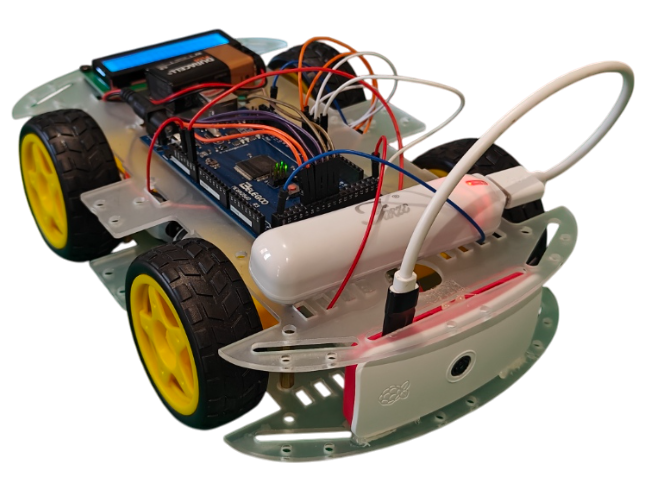
\includegraphics[width=0.7\linewidth]{racer.png}
\end{figure}


\newpage    

\tableofcontents

\newpage    

\section{Introduzione}
    Il progetto RACER si incentra sullo sviluppo da zero di una macchina a guida autonoma grazie alla combinazione del Microcontrollore \cite{arduinomega}
    Arduino Mega 2560 R3 (prodotto dalla Elegoo), il Microcomputer \cite{pizero} Raspberry Pi Zero 2W e il Modello Convoluzionale \cite{yolo} YoloV5s. 
    Sebbene non si tratti di una classica RC-Car, l'idea principale è sostituire il controllo umano e il Radiocomando con un sistema basato su una rete neurale e sulla computer vision tramite OpenCV. Questo sistema è in grado di osservare l'ambiente, rilevare enti e segnali stradali e analizzare le corsie per correggere automaticamente la direzione del veicolo.

    Un primo approccio ha portato il team ad utilizzare un ESP32-S3-N16R8 in combinazione con una camera OV5560. Purtoppo la bassa potenza di calcolo e la qualità costruttiva ci ha portato a sostituirlo con un Raspberry, in particolare l'antenna WiFi era debole, i contatti della camera estremamente sensibili che portavano a un degrado delle prestazioni con minimi movimenti e il corpo macchina della OV5560 tendeva a surriscaldarsi molto velocemente portando a un ulteriore degrado delle prestazioni.


\section{Progettazione del Veicolo}

\subsection{Arduino - Il cuore}

Alla base di ogni autovettura c'è sempre un motore, per RACER sono state utilizzati 4 piccoli motori DC a bassa tensione (9v) che possono essere controllati con i pin PWM di Arduino. In particolare la struttura è 4WD (Four Wheel Drive), ovvero a trazione integrale dove ogni ruota è motrice e può essere impostata autonomamente.

A disposizione avevamo un solo L293D (dual H-Bridge motor driver) per il controllo di direzione e velocità, sono quindi stati collegati in serie i 2 motori di destra e di sinistra. Ciò semplifica anche la gestione della svolta poichè per sterzare è necessario che i due motori di ambi i lati abbiano velocità equivalenti. I comandi che verranno gestiti sono Start, Stop, Sterzata a destra e sinistra e variazione di velocità a due livelli.
è stato inserito anche uno schermo LCD 16x2 che funge da debugger per comprendere in tempo reale cosa sta facendo l'Arduino.

Il "telaio" è in resina con ruote in gomma/plastica.



\begin{figure}[h!]
\centering
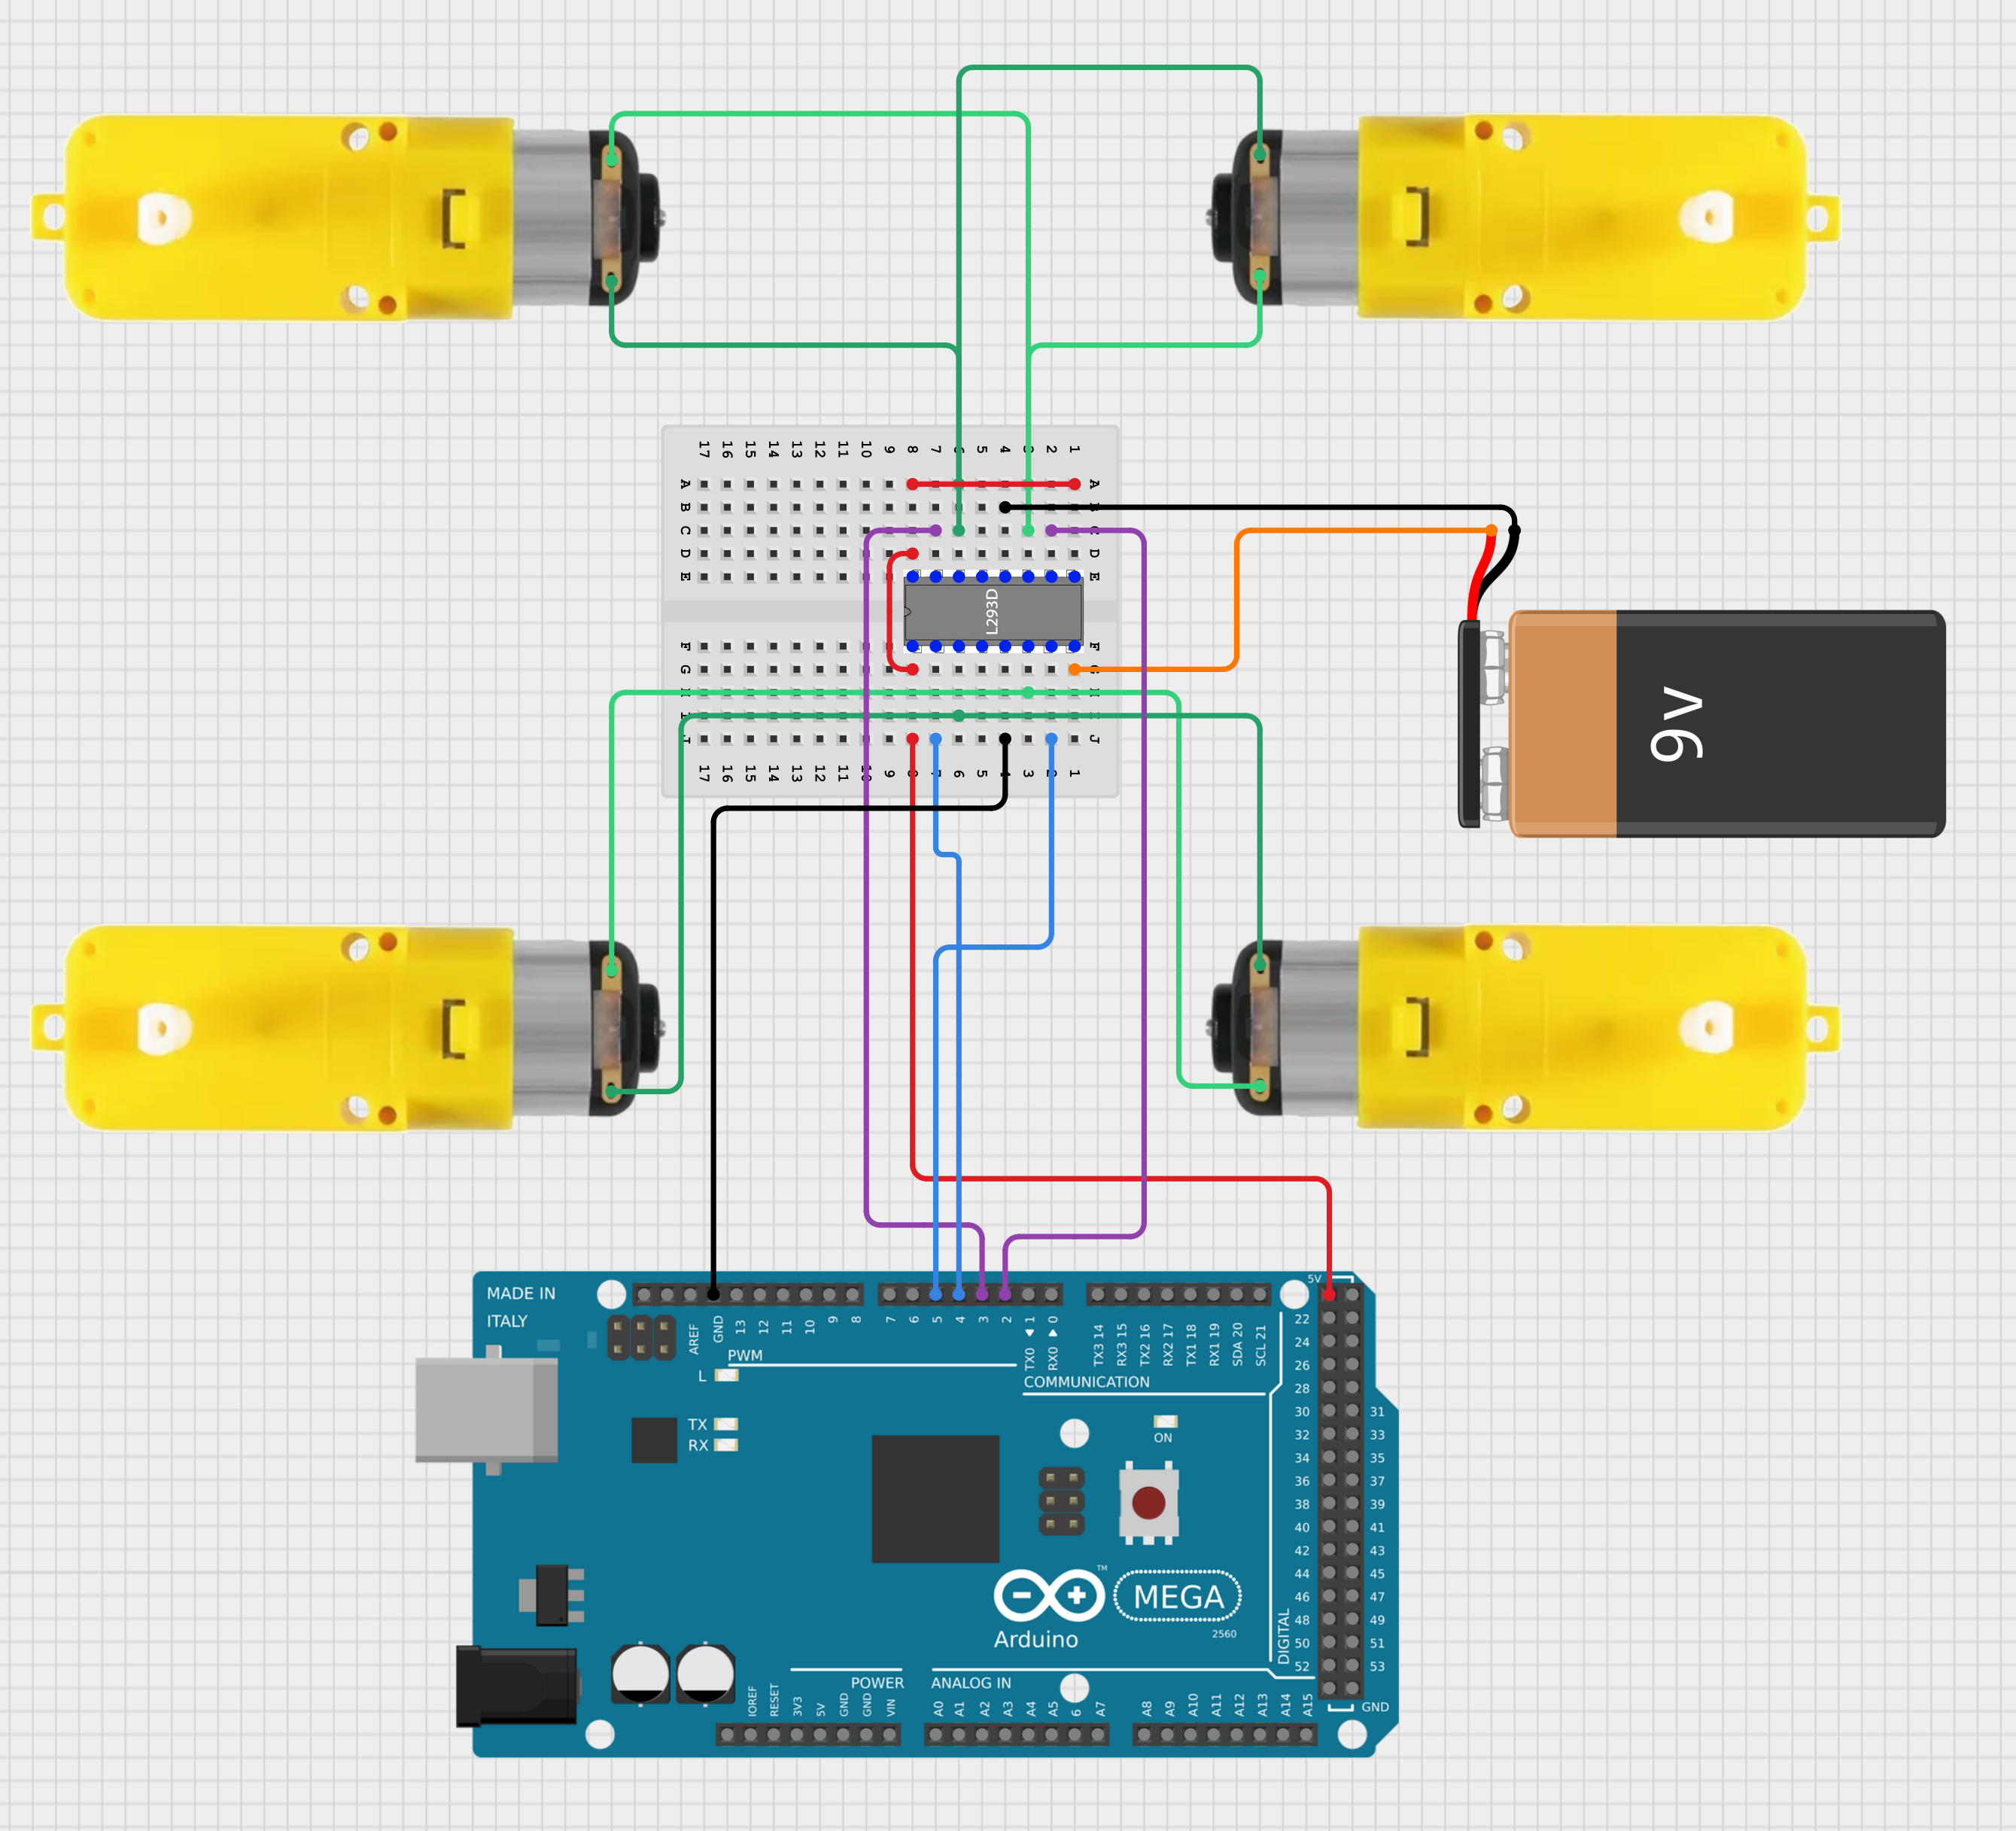
\includegraphics[width=0.65\linewidth]{Schema_Motori_Arduino.png}
\caption{Circuito completo dei motori.}
\end{figure}


\subsection{Raspberry Pi Z2W + PiCamera V2 - Gli occhi della macchina}

 Per catturare i dati ambientali abbiamo utilizzato un Raspberry Pi Z2W, dotato di processore Quad-core Cortex-A53 a 1.0 GHz a 64bit e 512MB LPDDR2 di RAM, in combinazione con una \cite{picamera} PiCamera V2 che monta un sensore Sony IMX219 da 8 Megapixel. Entrambi i componenti sono stati montati in un case apposito della Raspberry mostrato in figura e montato nella parte anteriore del veicolo.

Questo modulo si occuperà di:
\begin{itemize}
\item Catturare un flusso video 720x1280 e streammarlo su una rete locale (Hotspot Cellulare). Lo streaming sarà in contemporanea catturato mediante OpenCV su un PC che sta eseguendo il programma principale di analisi ambientale.
\item Gestire connessioni TCP con un terminale per lo scambio di messaggi.
\item Inoltro dei comandi ad Arduino.
\end{itemize}

\subsection{Comunicazione tra i moduli}
\begin{enumerate}
\item PC collegato alla stessa rete del Raspberry cattura con OpenCV lo streaming video.
\item  Con la libreria Socket invierà i comandi/messaggi utilizzando il protocollo TCP su porta 5005 al Raspberry.
\item Una volta ricevuti, il Raspberry li inoltrerà all'Arduino tramite il collegamento UART0 (Universal Asynchronous Receiver-Transmitter) che permette lo scambio su porta seriale in modo asincrono. Abbiamo deciso di rendere la comunicazione unidirezionale, solo il Pi invia Pin TX Pi - Pin Rx Arduino.  
\begin{figure}[h!]
  \centering
  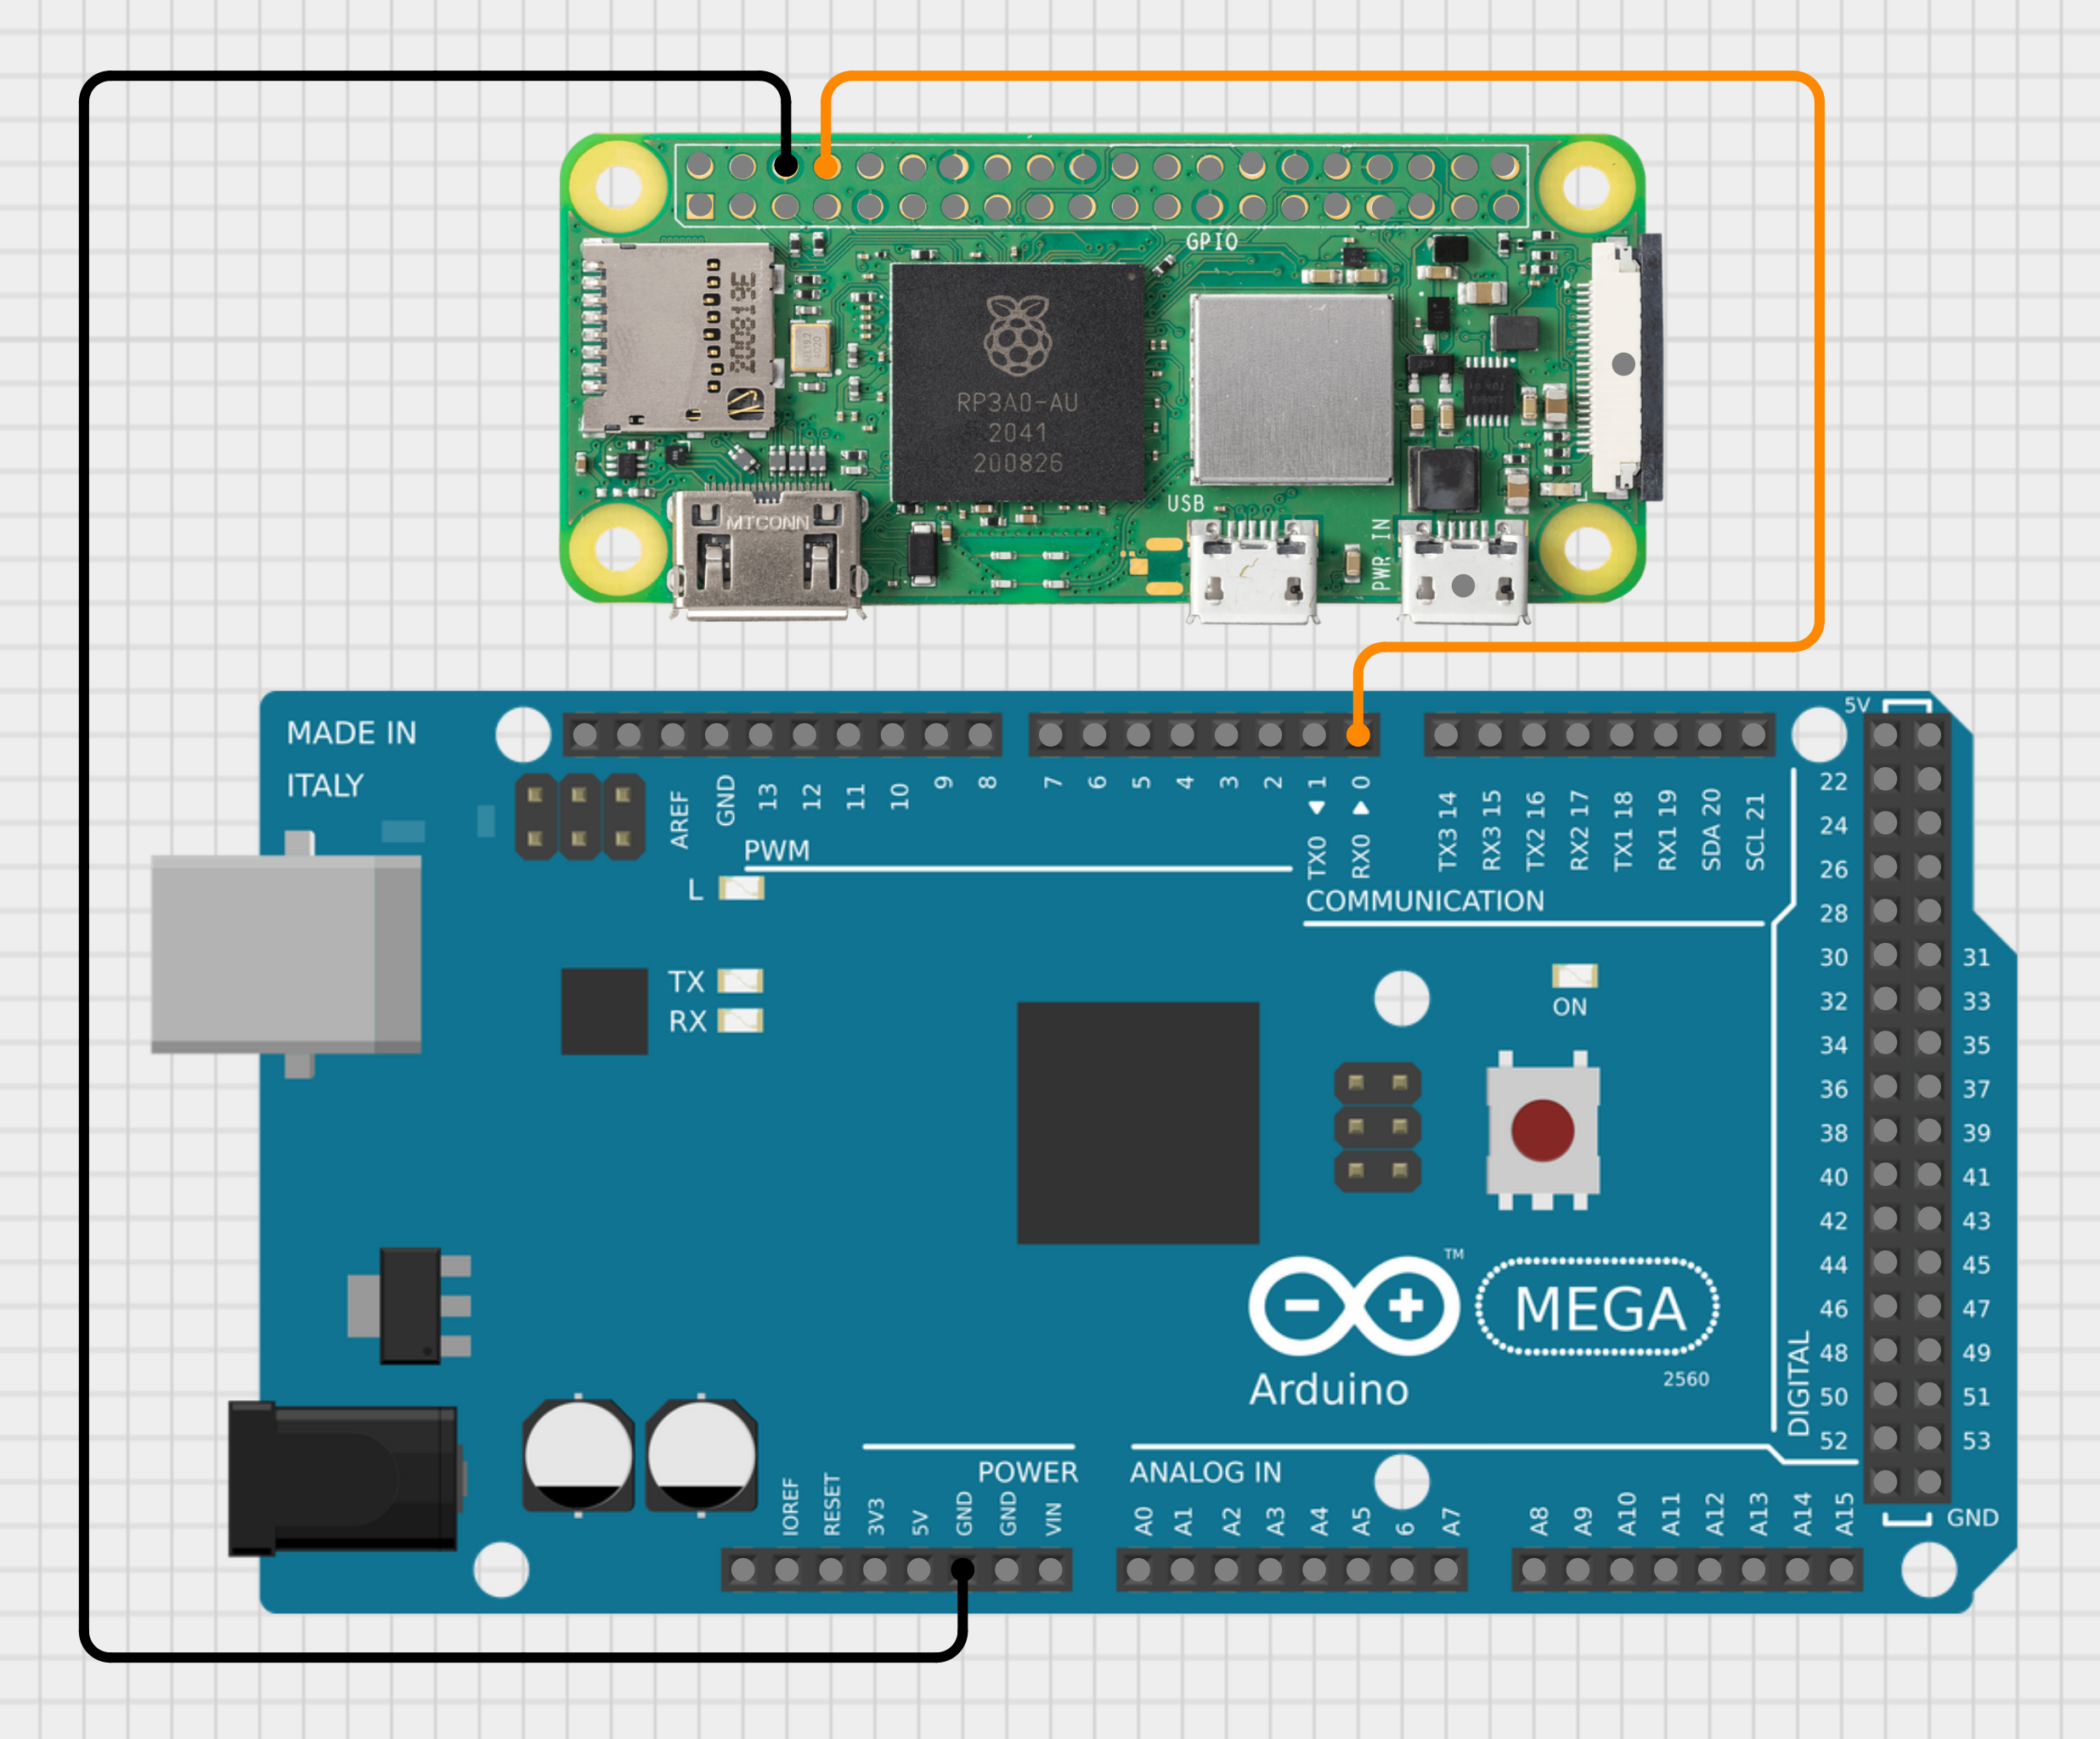
\includegraphics[width=0.5\textwidth]{uart0.png}
    \caption{Collegamento UART}
\end{figure}

\item \cite{flaskstream} Streaming Video Raspberry

    Abbiamo creato un'app WebCamera Server utilizzando il framework Flask e le librerie PiCamera2 e OpenCV per catturare i frame dalla PiCamera. L'app si occupa di inviare il flusso di frame catturato dalla camera al dispositivo connesso su porta 8080.
    Successivamente abbiamo reso lo script in un servizio linux, in modo che venga eseguito in automatico all'accensione. Per la realizzazione dell'app ci siamo affidati alla seuente \href{https://github.com/miguelgrinberg/flask-video-streaming/tree/v1}{repository}. 
\end{enumerate}

\newpage

\subsection{Alimentazione}
\begin{itemize}
\item Arduino: Batteria 9v.
\item Motori: Batteria 9v.
\item Raspberry: Powerbank 5V/1A.
\end{itemize}

\section{Sviluppo Software}
\subsection{Introduzione}
Il programma di elaborazione dei frame sfrutta il \cite{multithreading} multithreading per ottenere prestazioni ottimali e fluide e si suddivide come segue:

\begin{itemize}
    \item Thread Principale: Esegue la Lane Daetection e invia i comandi relativi a direzione e ciò che Yolo ha individuato solo se il Thread1 ha acquisito il frame.
    \item Thread1: Si occupa di acquisire i frame. 
    \item Thread2: Esegue l'inferenza di Yolo e salva le classi immagazzinate
\end{itemize} 

Di seguito è rappresentato il flusso di computazione semplificato:
\textit{Thread1 Frame Acquisito  $\rightarrow$ Thread2 Ogetti individuati nel frame $\rightarrow$ Thread Principale Lane Detection + Invio Comandi}  


\subsection{YoloV5s - Il Cervello}
    
    \subsubsection{Cosa è YoloV5}
    \cite{yolov5arch}
    YOLO (You Only Look Once) è una serie di modelli di riconoscimento degli oggetti in tempo reale basato sulla rete neurale convoluzionale. Il suo nome fa riferimento alla caratteristica che lo contraddistingue da modelli simili precedenti, ovvero che il modello richiede un solo passaggio di propagazione in avanti per poter fare delle previsioni.
    Il modello è stato creato da Joseph Redmon, che ha sviluppato le prime tre versioni e pubblicate sul suo sito web. Successive versioni sono state sviluppate da altri enti, la versione utilizzata da noi (v5) ad esempio è stata sviluppata dalla Ultralytics.
    
    \subsubsection{Architettura}
    \cite{yolotutorial}  \cite{yoloarch}
    Modelli di riconoscimento di oggetti classici richiedono due passaggi dell'immagine in input, la prima per generare un insieme di potenziali posizioni di oggetti (proposte), la seconda serve per raffinare tali proposte e ottenere le previsioni finali.
    Inoltre, alcuni modelli, come del tipo Region Proposal Networks, eseguono diverse istanze del modello per una singola immagine, una per ogni regione separatamente. Tutto ciò richiede una quantità di risorse considerevole.
    Il modello YOLO esegue un singolo passaggio dell'immagine in input sia per le proposte e sia per la previsione finale, inoltre esegue le previsioni sull'immagine in input nella sua interezza nello stesso momento, grazie all'uso di un singolo layer completamente connesso. 
    Infine, la struttura stessa di YOLO è relativamente semplice: una singola rete convoluzionale esegue le previsioni sia delle classi sia dei bounding box. Questo è possibile grazie ad un approccio differente ed innovativo di YOLO rispetto ad algoritmi precedenti, che sono essenzialmente dei modelli di classificazione modificati per la rilevazione di oggetti.
    La rete convoluzionale di YOLO viene suddivisa in tre parti: 
    \begin{itemize}
        \item Backbone: che è responsabile dell'estrazione delle caratteristiche dall'immagine di input.
        \item Neck: che esegue trasformazioni sulle caratteristiche estratte dalla Backbone
        \item Head: che si occupa delle previsioni finali.
    Versioni successive di YOLO sono aggiornamenti e modificazioni di questi tre moduli.
    \end{itemize}
    
\begin{figure}[h!]
    \centering
    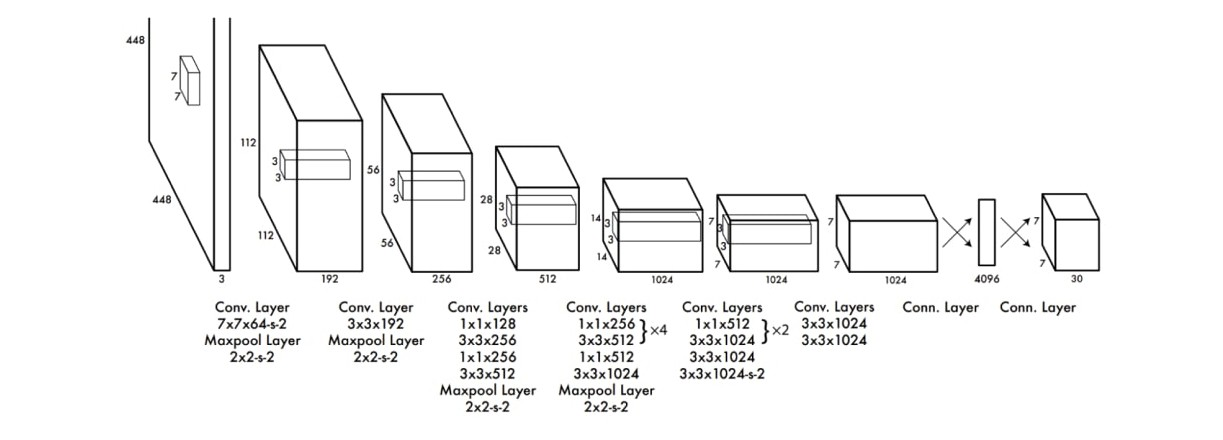
\includegraphics[width=1.1\linewidth]{architetttura_yolo.jpg}
    \caption{Architettura YoloV5}
\end{figure}

\newpage
YOLO divide l'immagine in input in una griglia SxS. Se il centro di un oggetto si trova dentro una cella, quella cella si occuperà di rilevare quell'oggetto.
Ogni cella prevede B bounding box e un punteggio di confidenza per ognuno di quei box. La confidenza quantifica la probabilità di quel box di contenere un oggetto e con quale precisione. Inoltre ad ogni cella prevede C probabilità di classe, ovvero che tipo di oggetto si trova dentro la cella. 
Queste due informazioni vengono unite per produrre le previsioni finali.

\begin{figure}[h!]
    \centering
    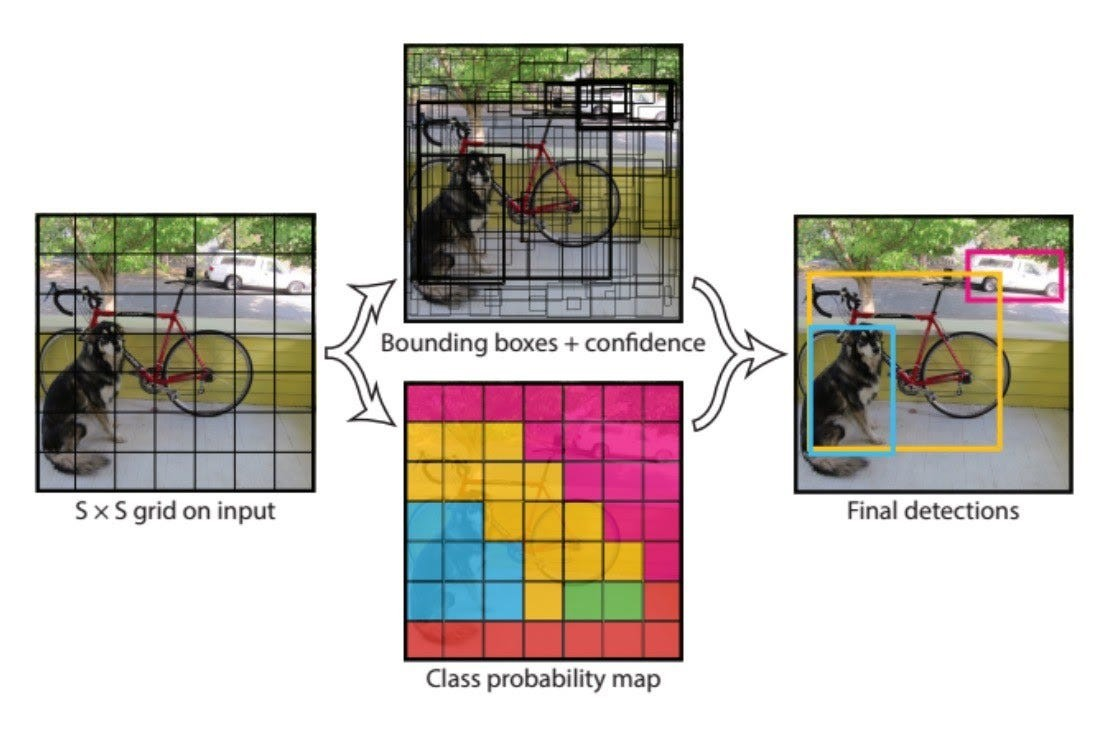
\includegraphics[width=0.8\linewidth]{cf.jpg}
    \caption{Tiling Input}
\end{figure}

\subsubsection{Perchè lo abbiamo scelto}
Grazie a questo, YOLO è estremamente veloce, in grado di elaborare un flusso di immagini in tempo reale con bassissima latenza, pur mantenendo un alta precisione, e ciò è proprio il nostro caso di utilizzo: l'automobile deve riconoscere rapidamente i vari ostacoli e situazioni che si presentano lungo la strada, ed attuare strategie di correzione tempestivamente.

\subsubsection{Training}


\begin{figure}[h!]
  \centering
  \begin{subfigure}[b]{0.495\textwidth}
    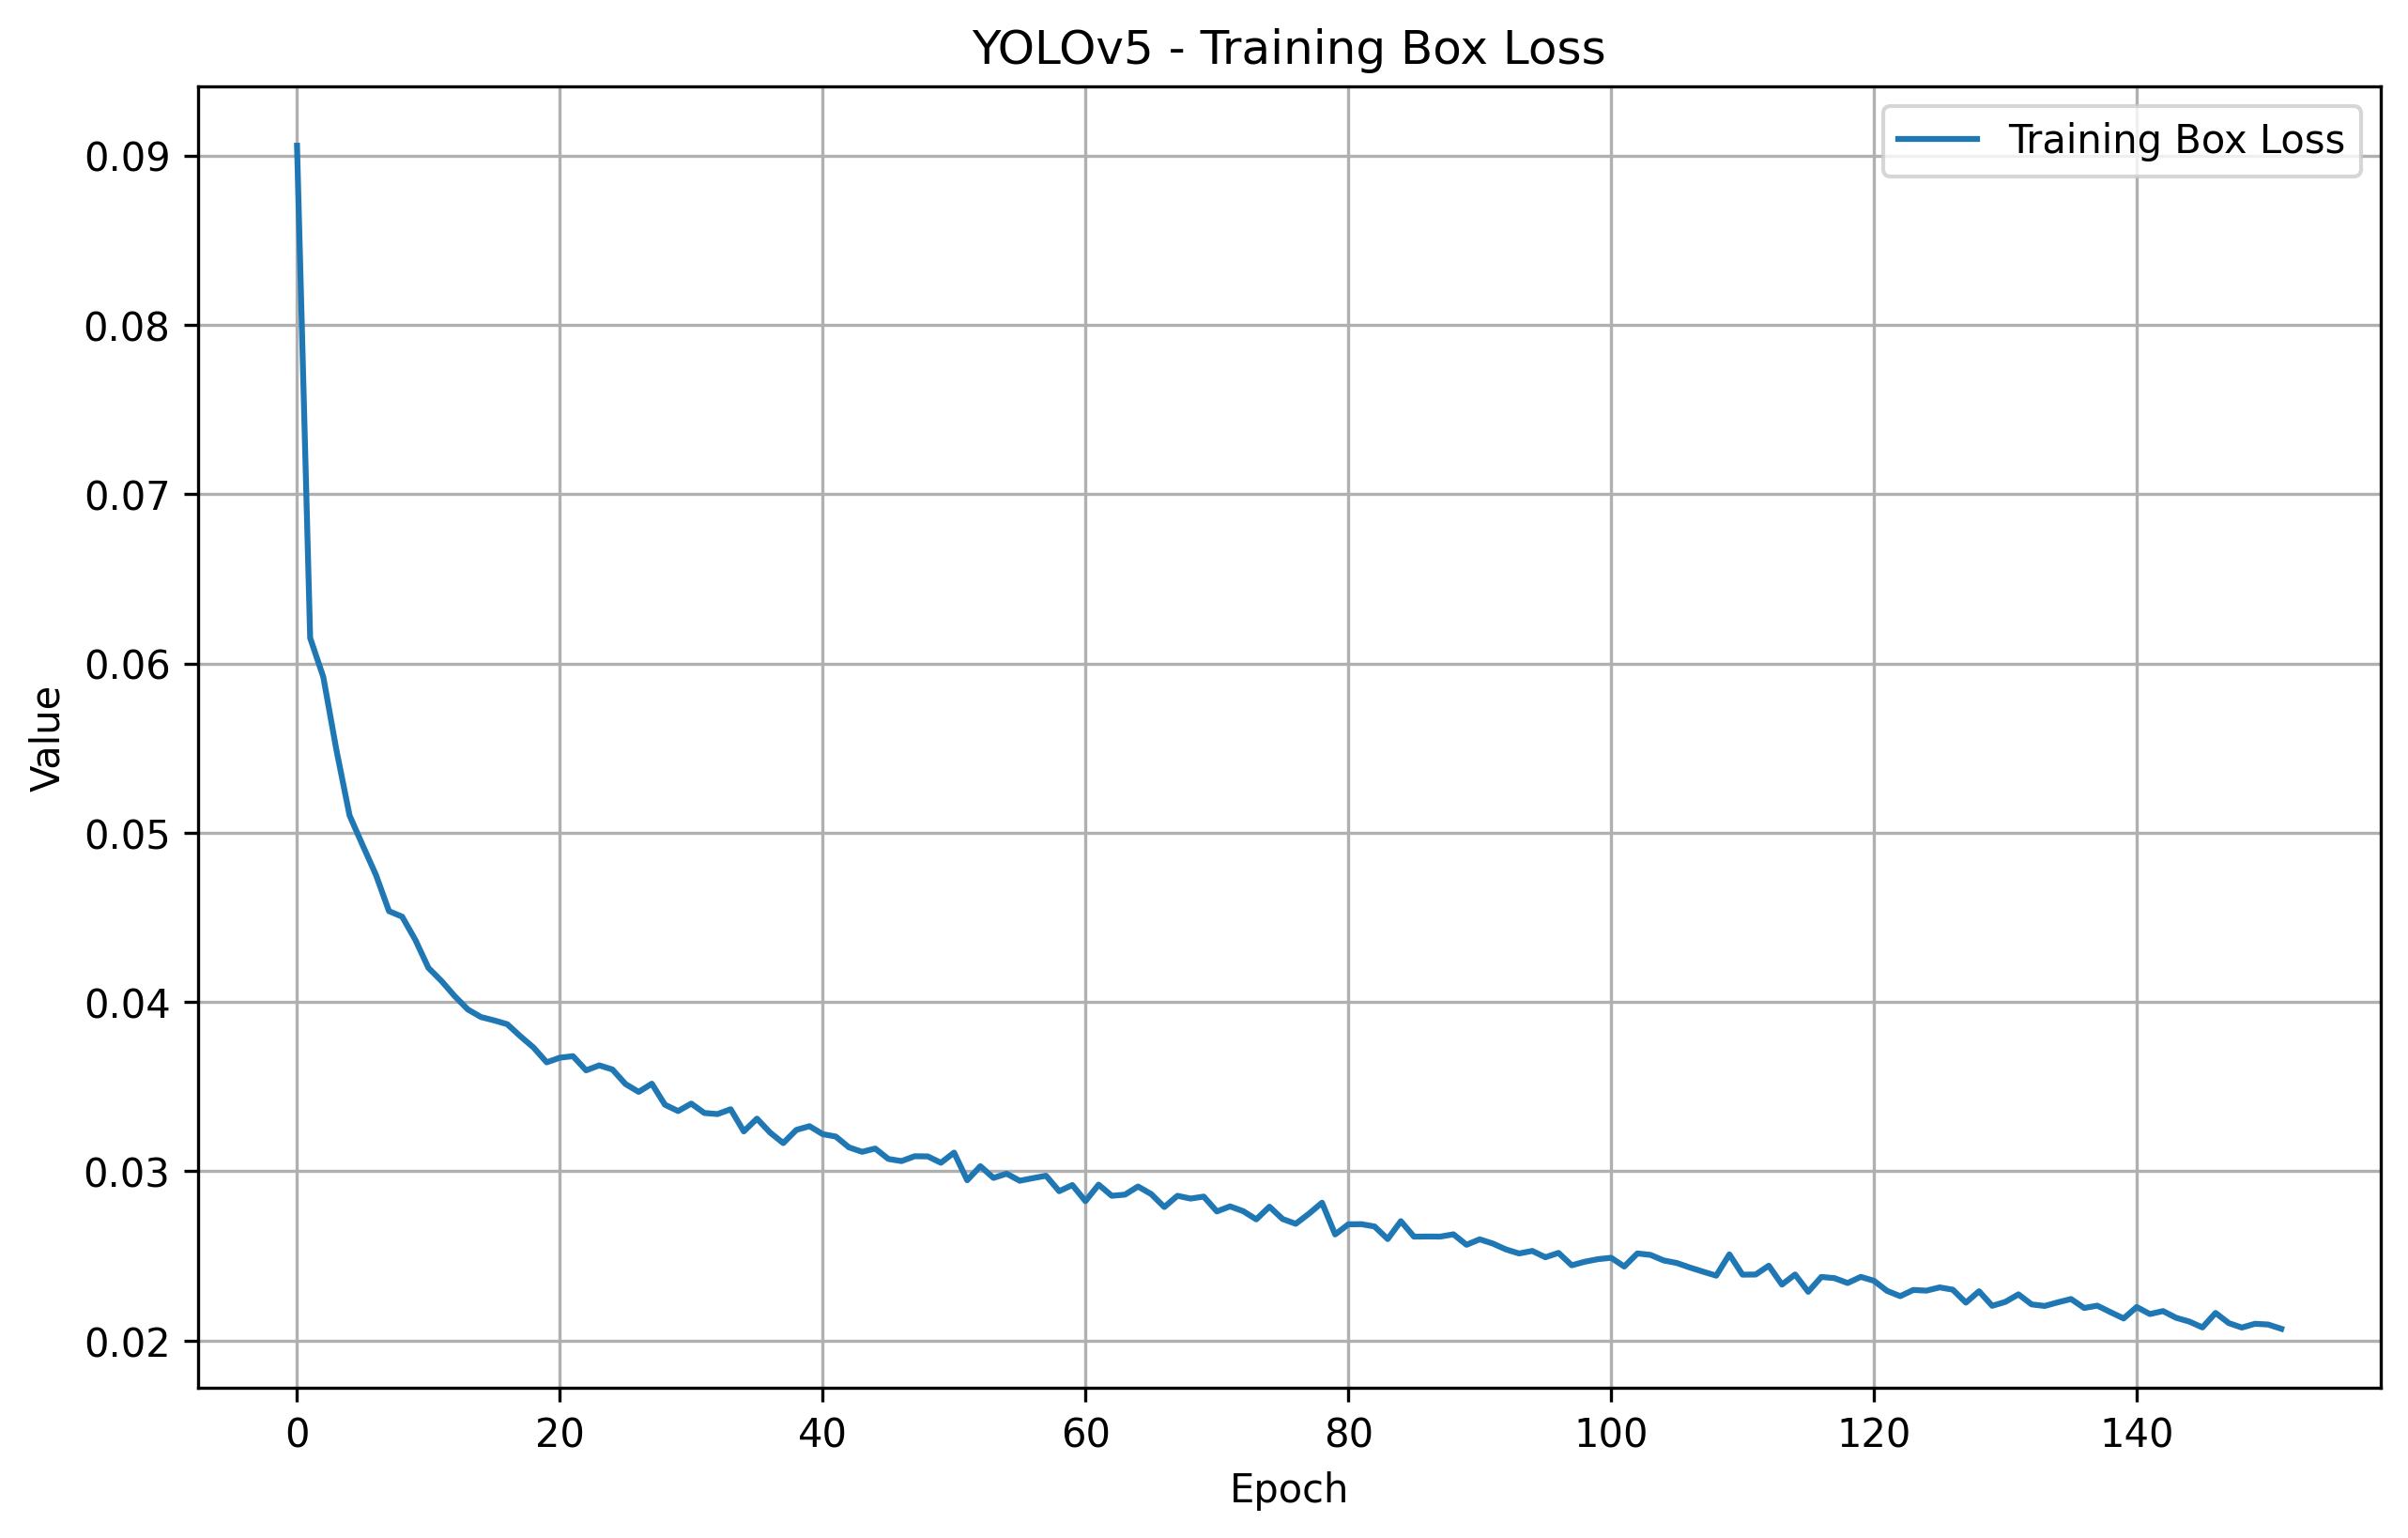
\includegraphics[width=\linewidth]{Training Box Loss.png}
    \caption{Box Loss}
  \end{subfigure}
  \begin{subfigure}[b]{0.495\textwidth}
    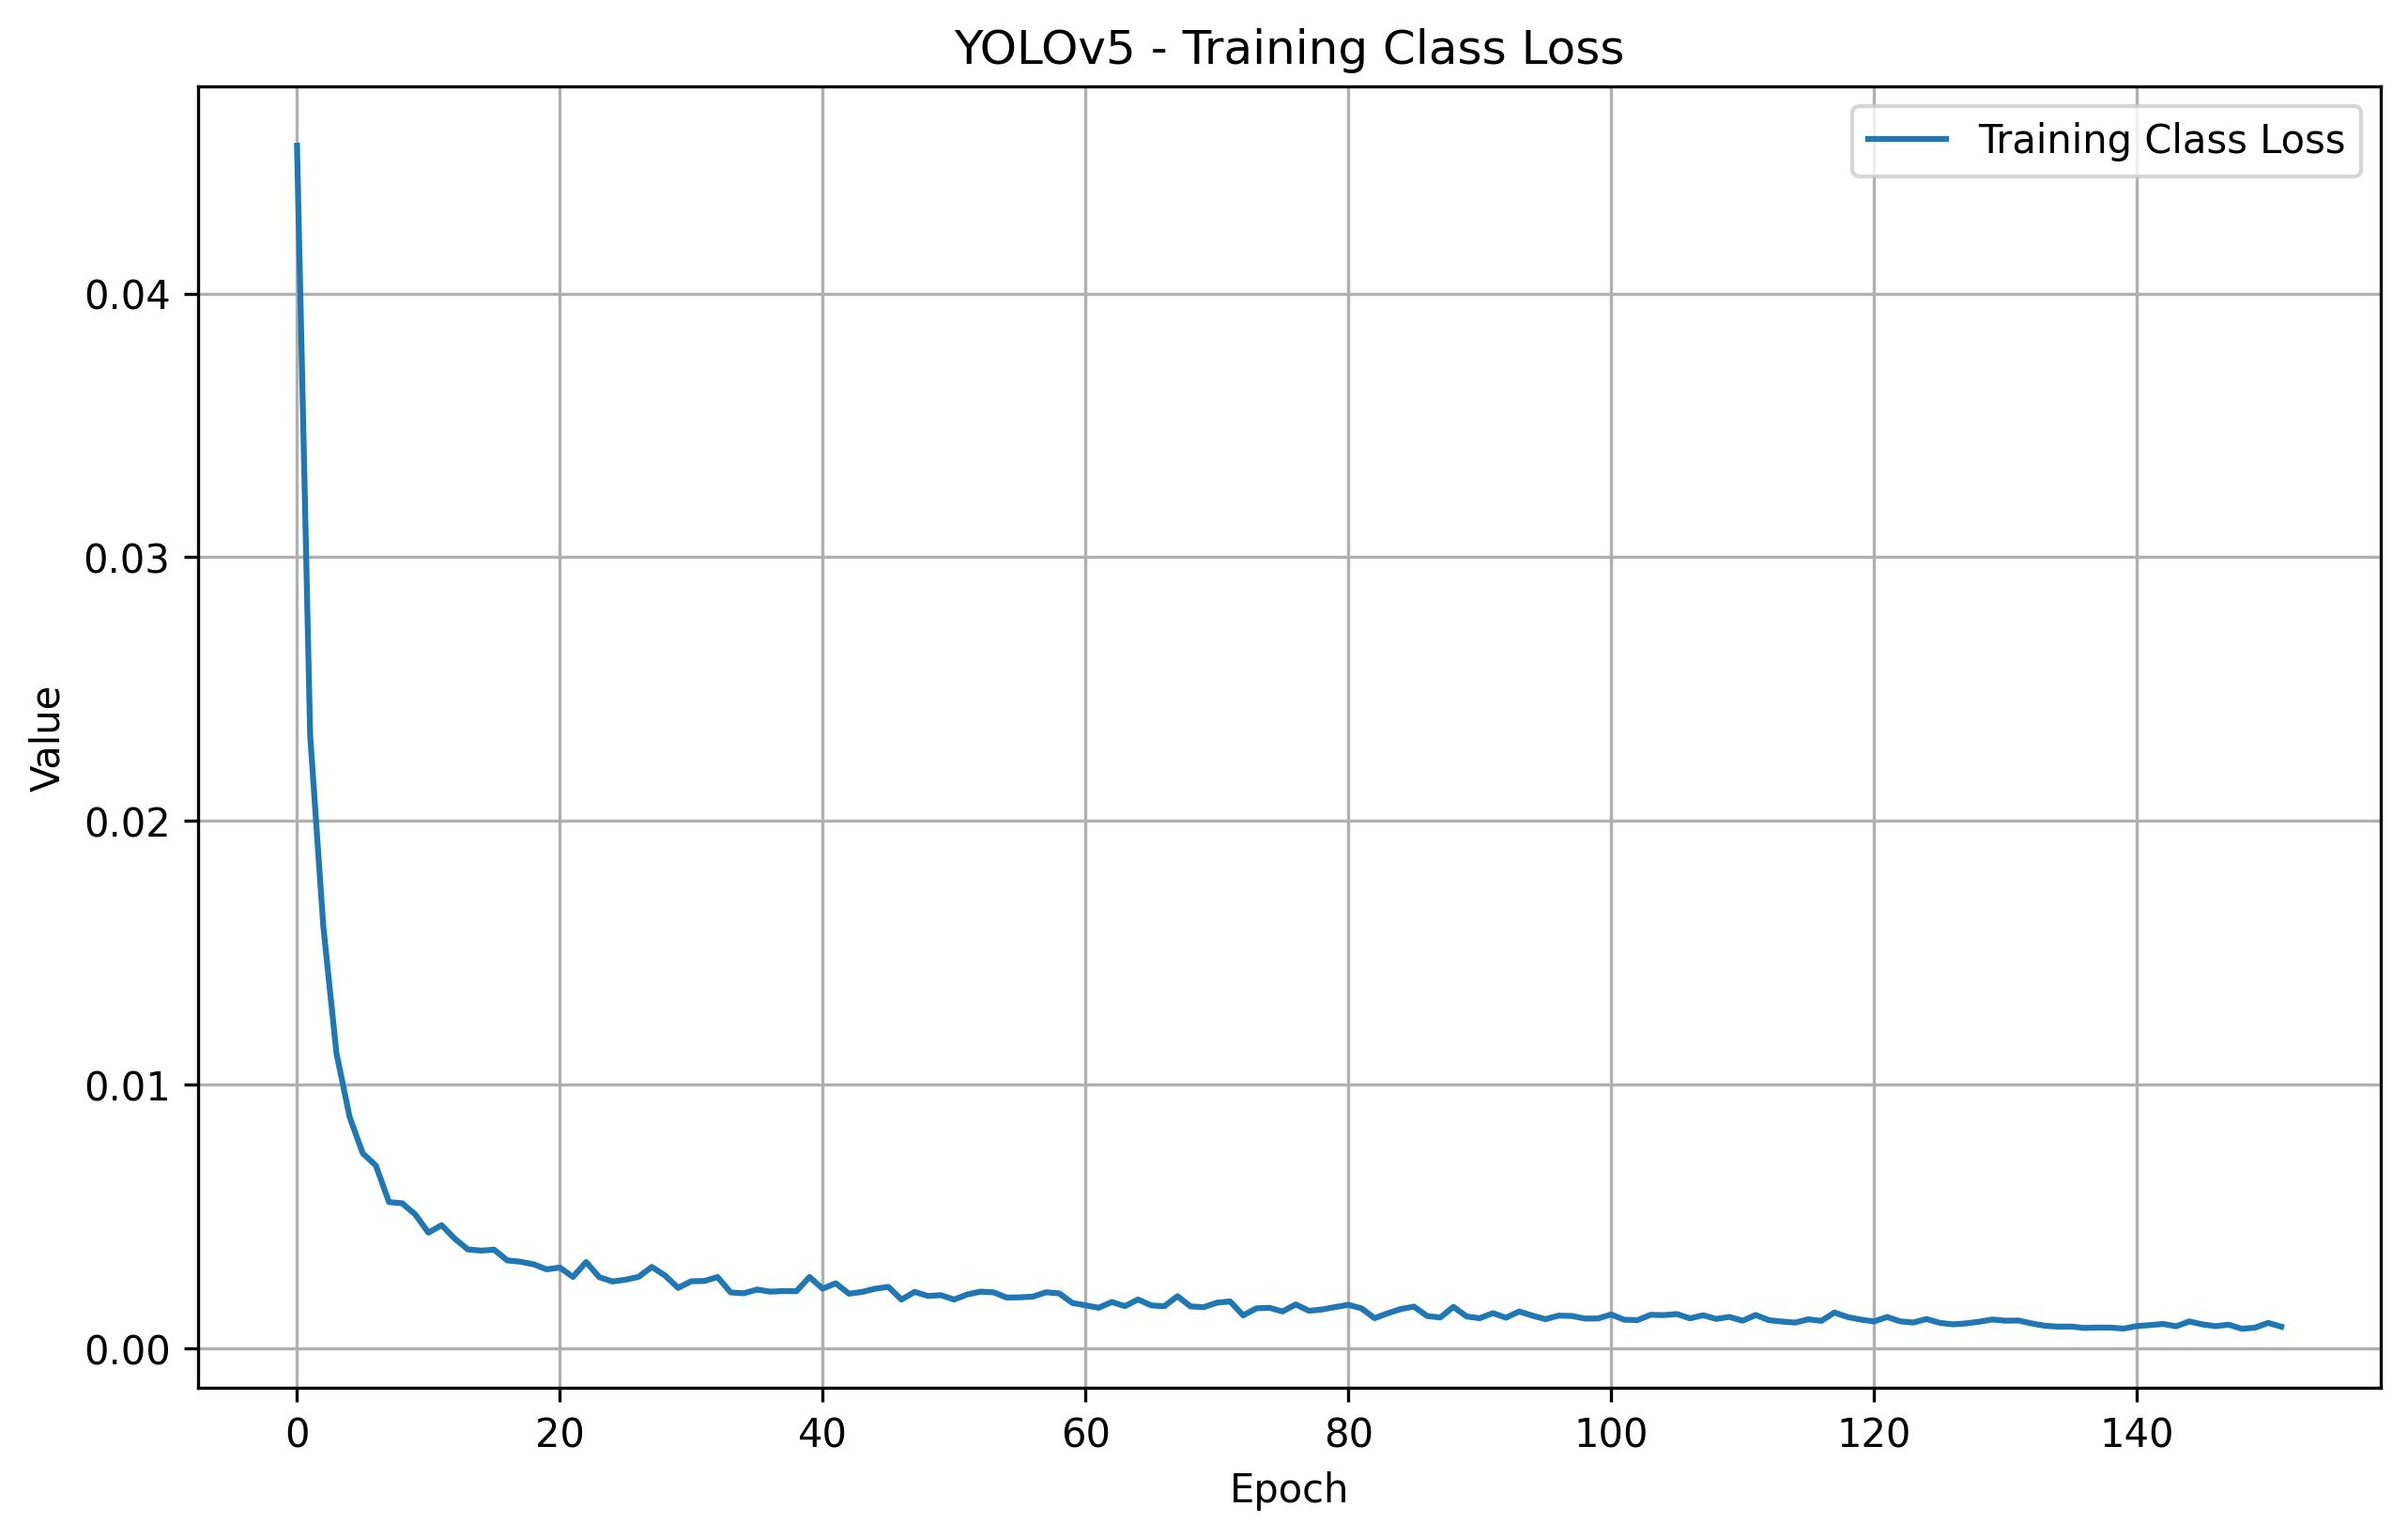
\includegraphics[width=\linewidth]{Training Class Loss.png}
    \caption{Class Loss}
  \end{subfigure}
\end{figure}

\begin{figure}[h!]
  \centering
  \begin{subfigure}[b]{0.495\textwidth}
    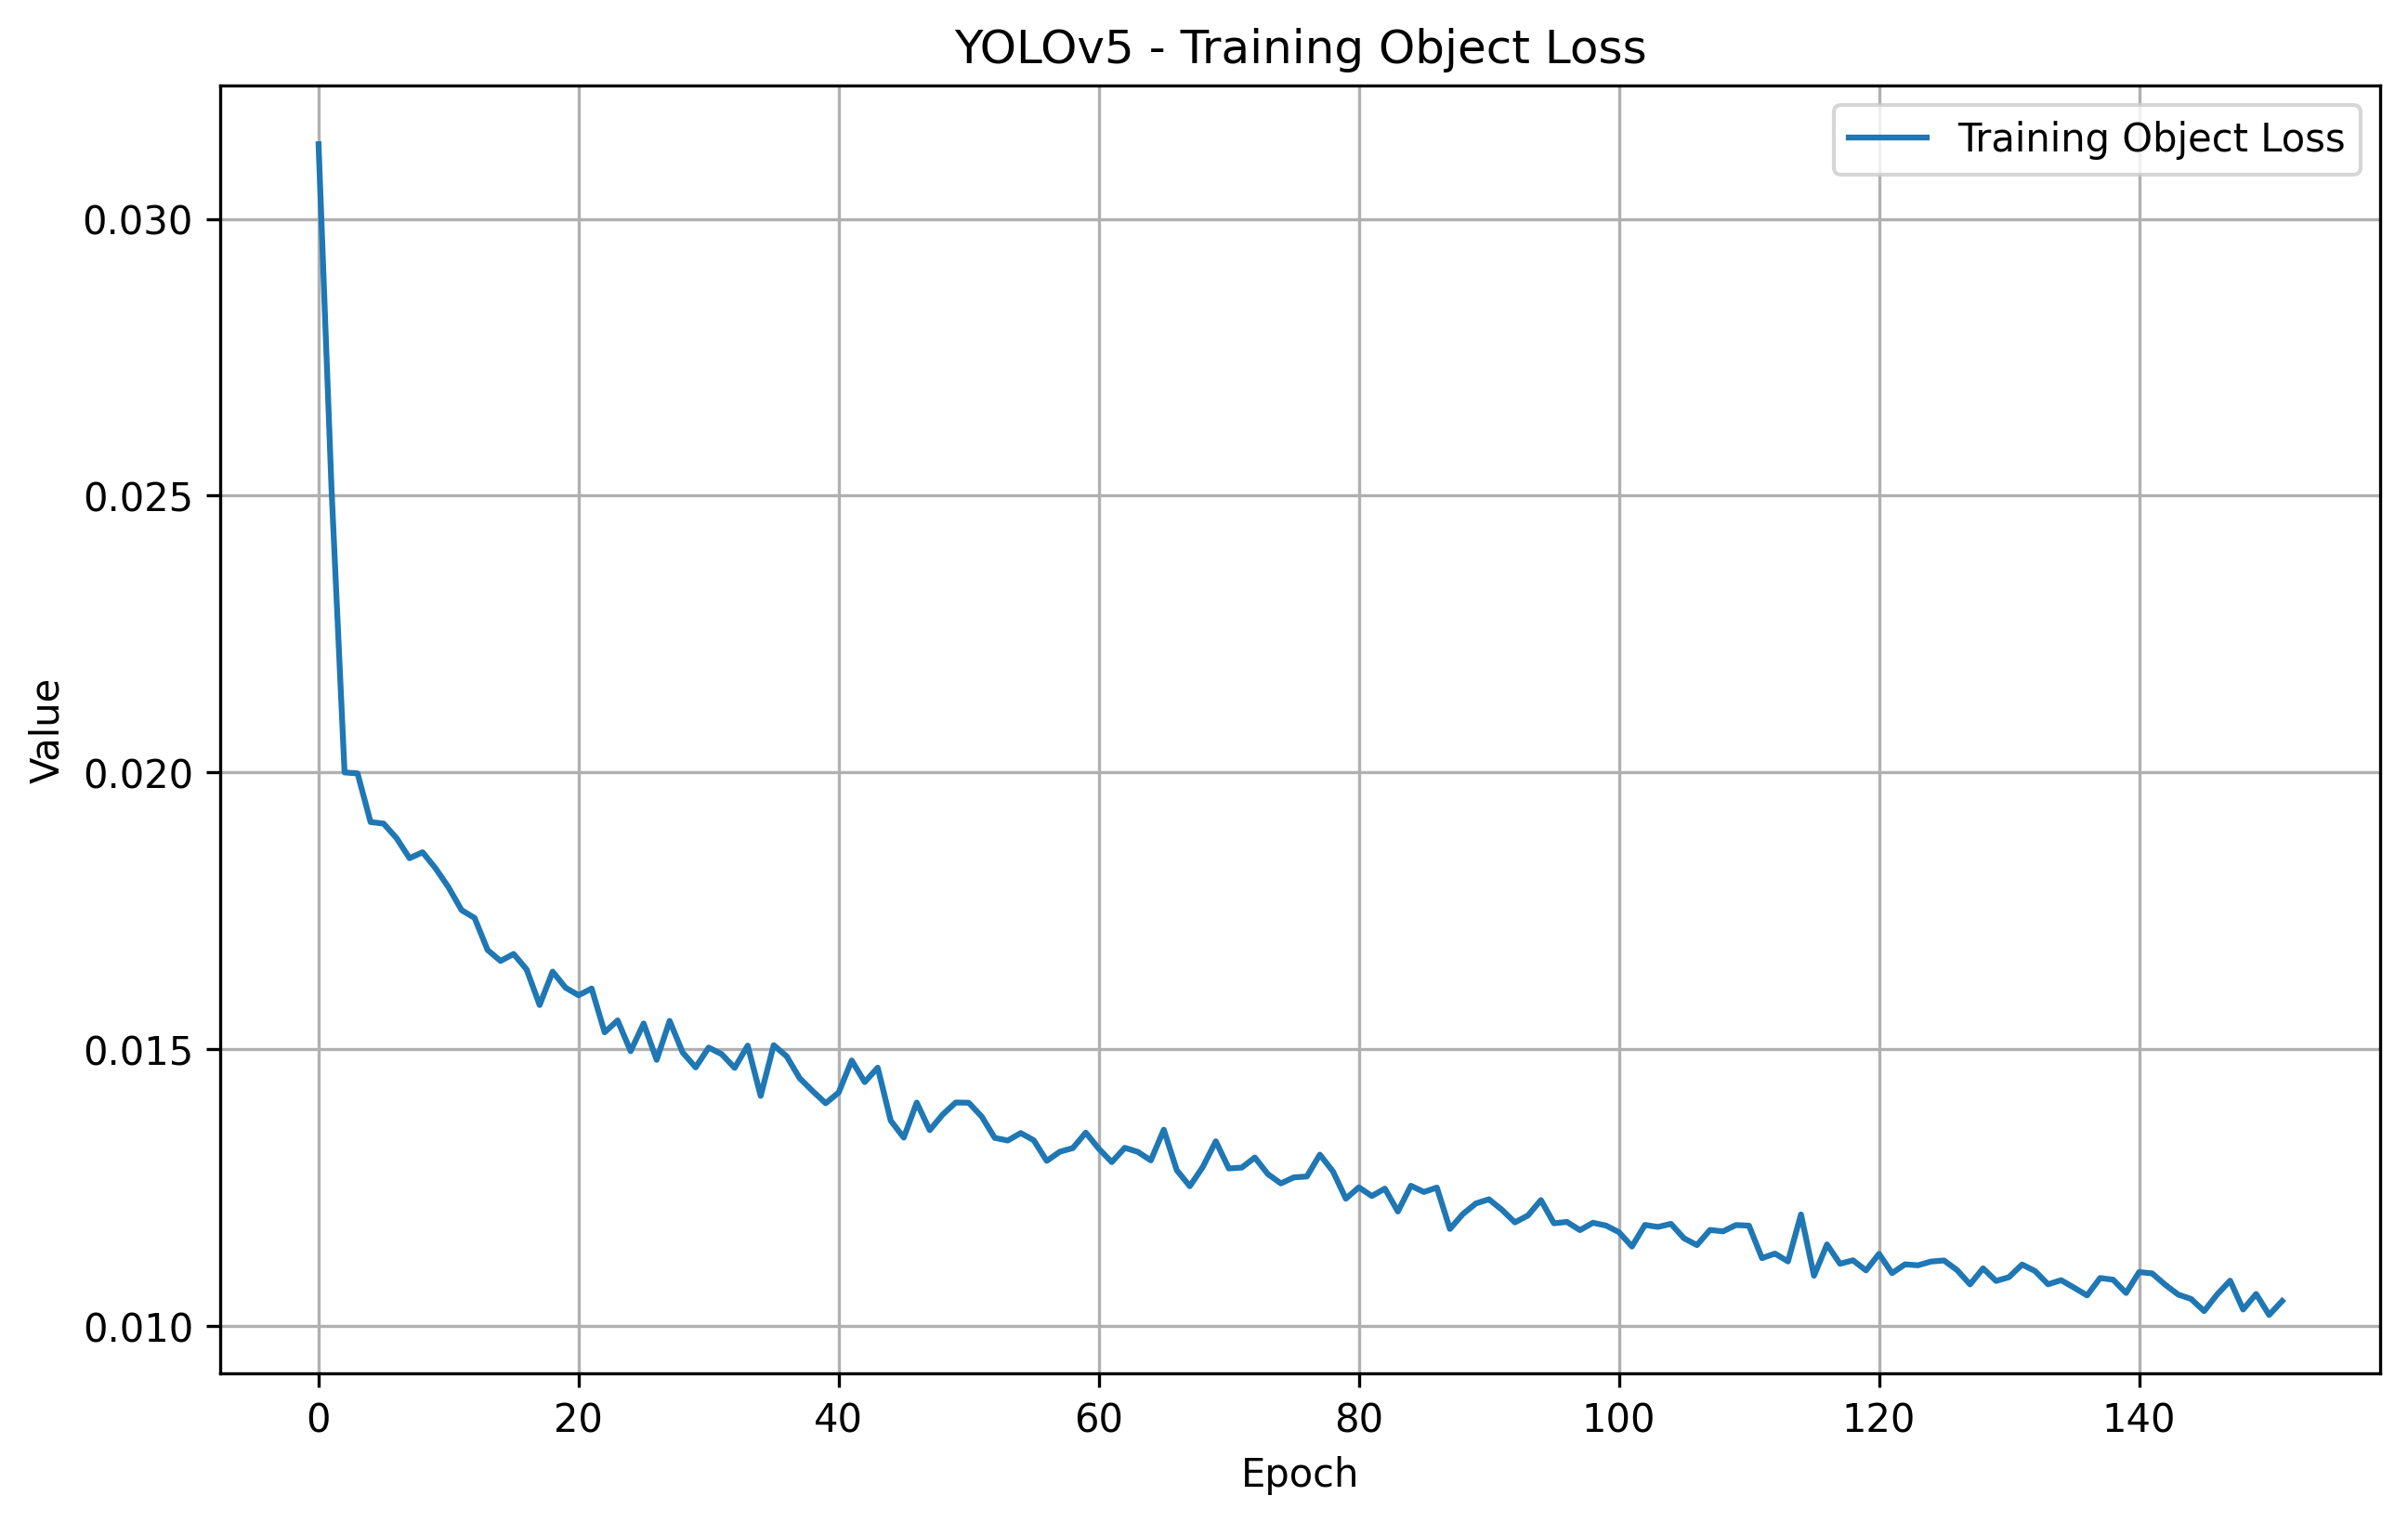
\includegraphics[width=\linewidth]{Training Object Loss.png}
    \caption{Box Loss}
  \end{subfigure}
  \begin{subfigure}[b]{0.495\textwidth}
    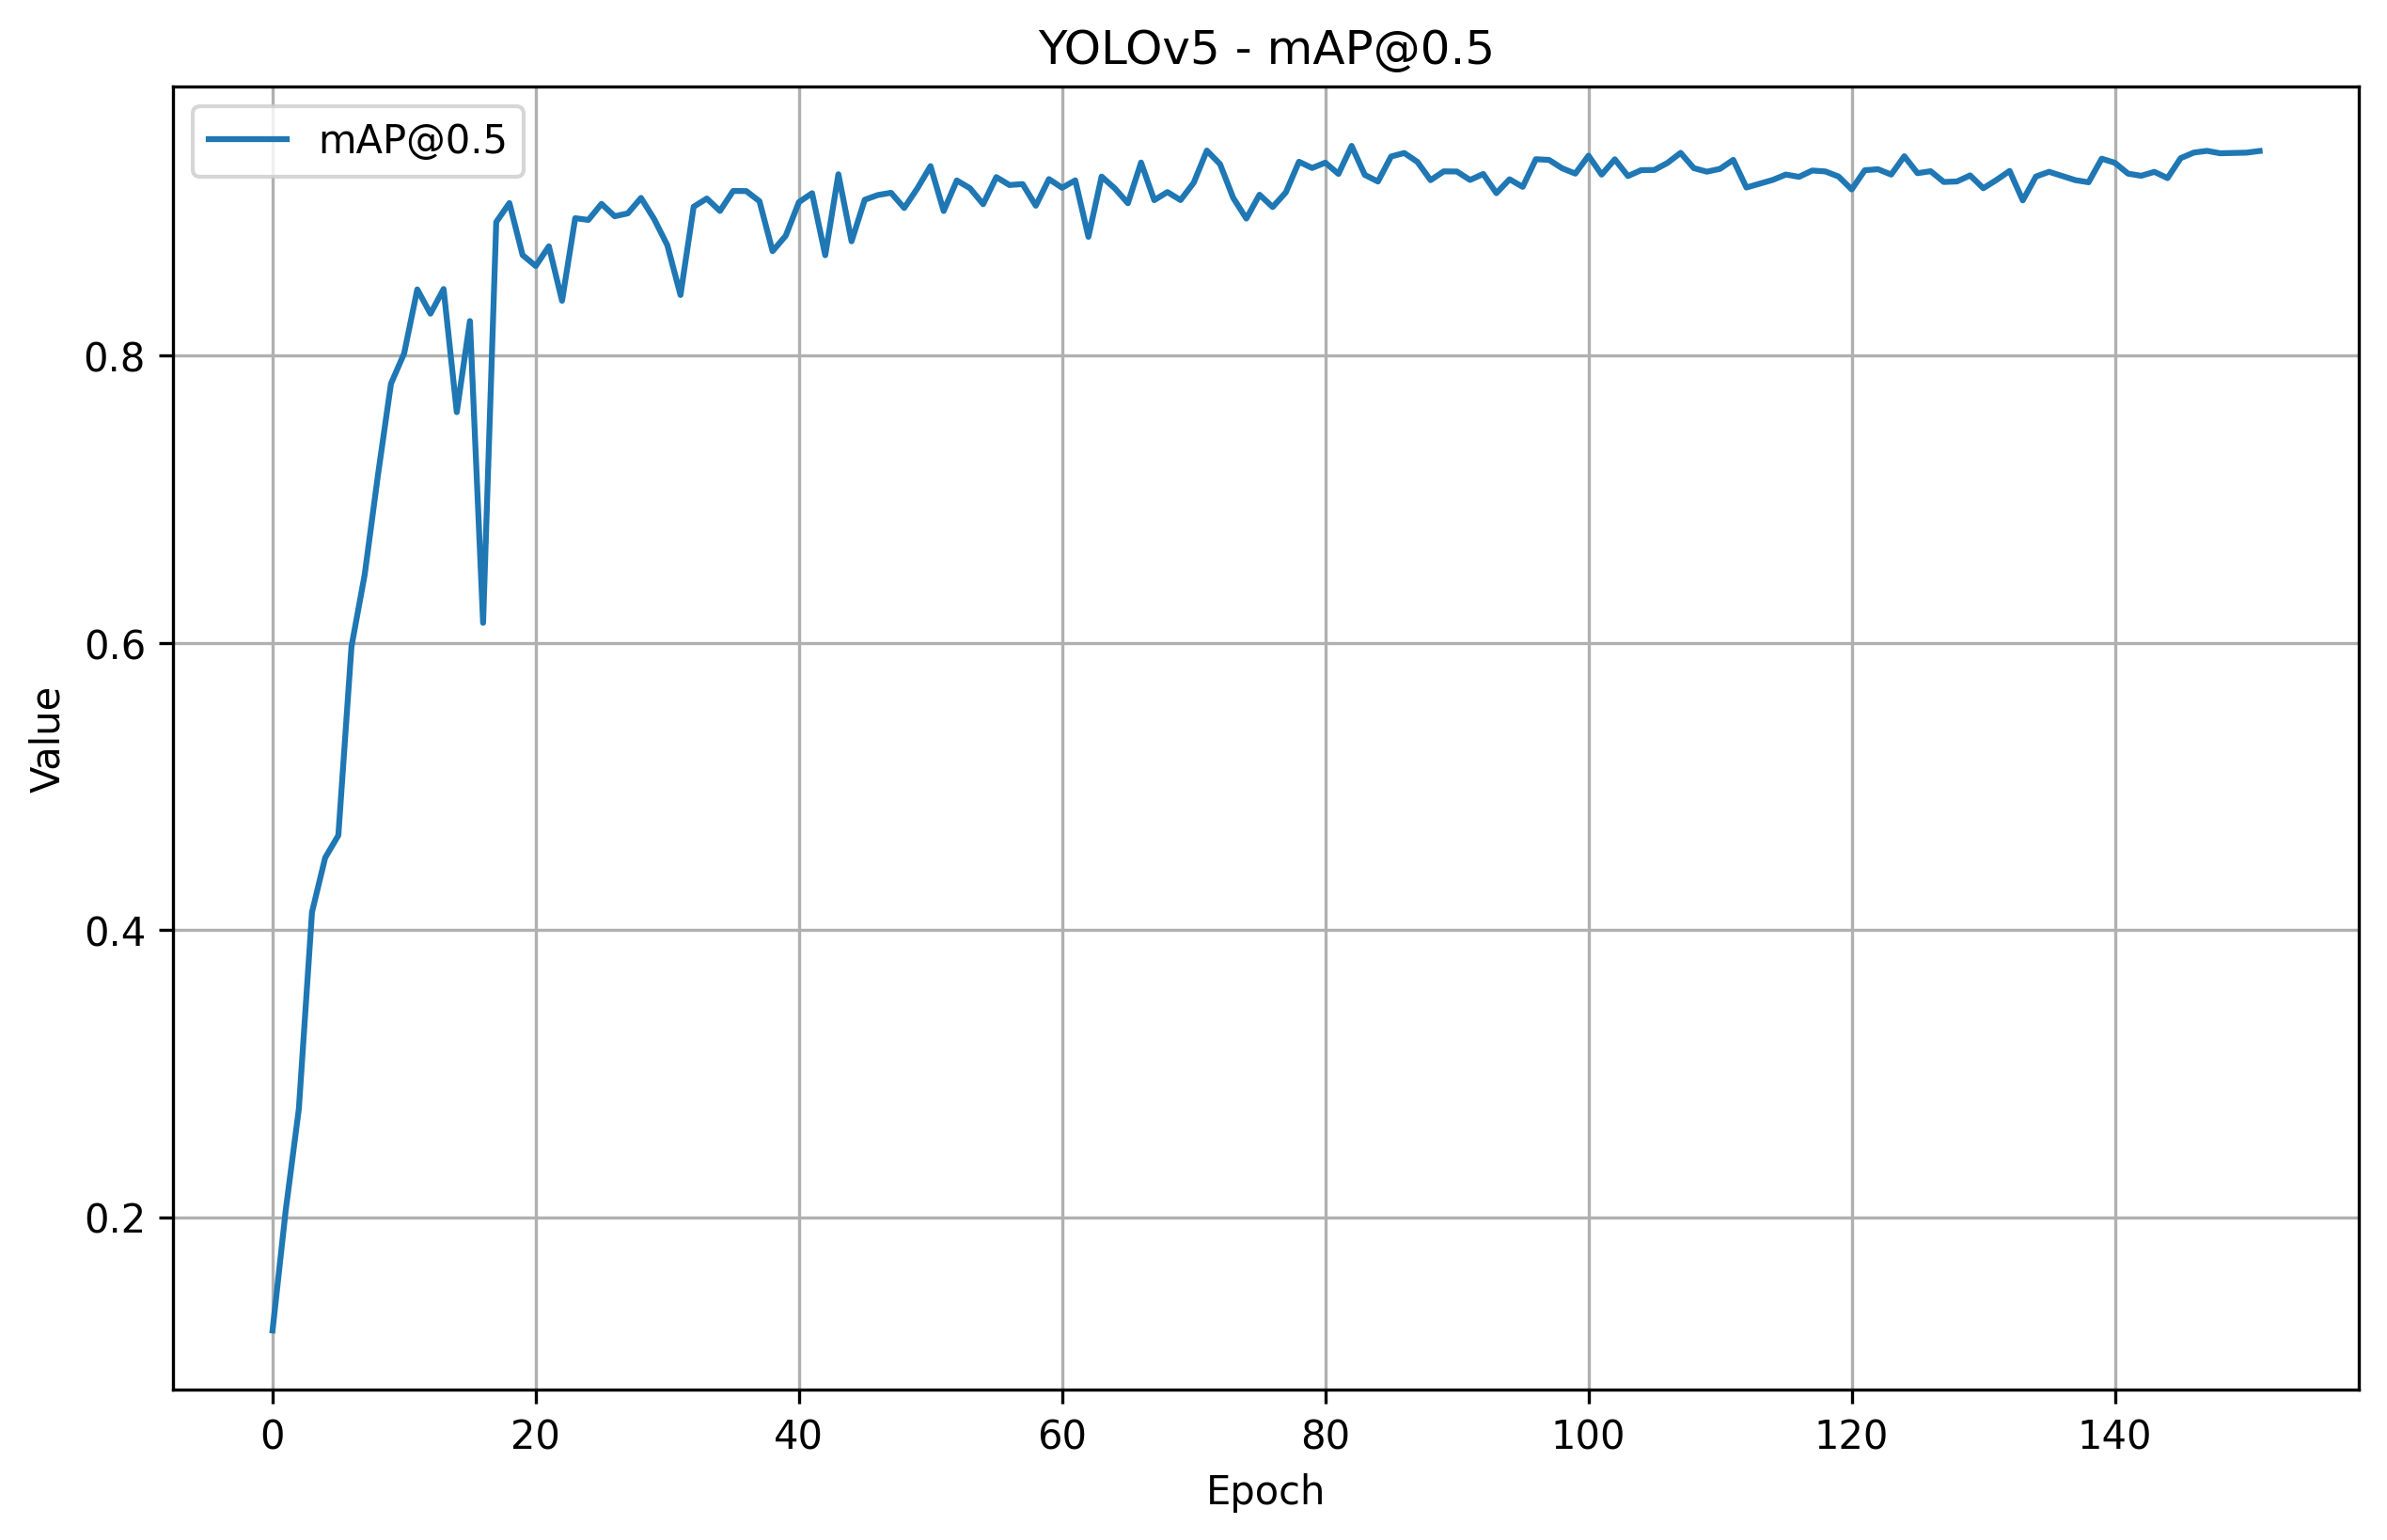
\includegraphics[width=\linewidth]{mAP_0.5.png}
    \caption{Class Loss}
  \end{subfigure}
\end{figure}

\begin{figure}[h!]
  \centering
  \begin{subfigure}[b]{0.495\textwidth}
    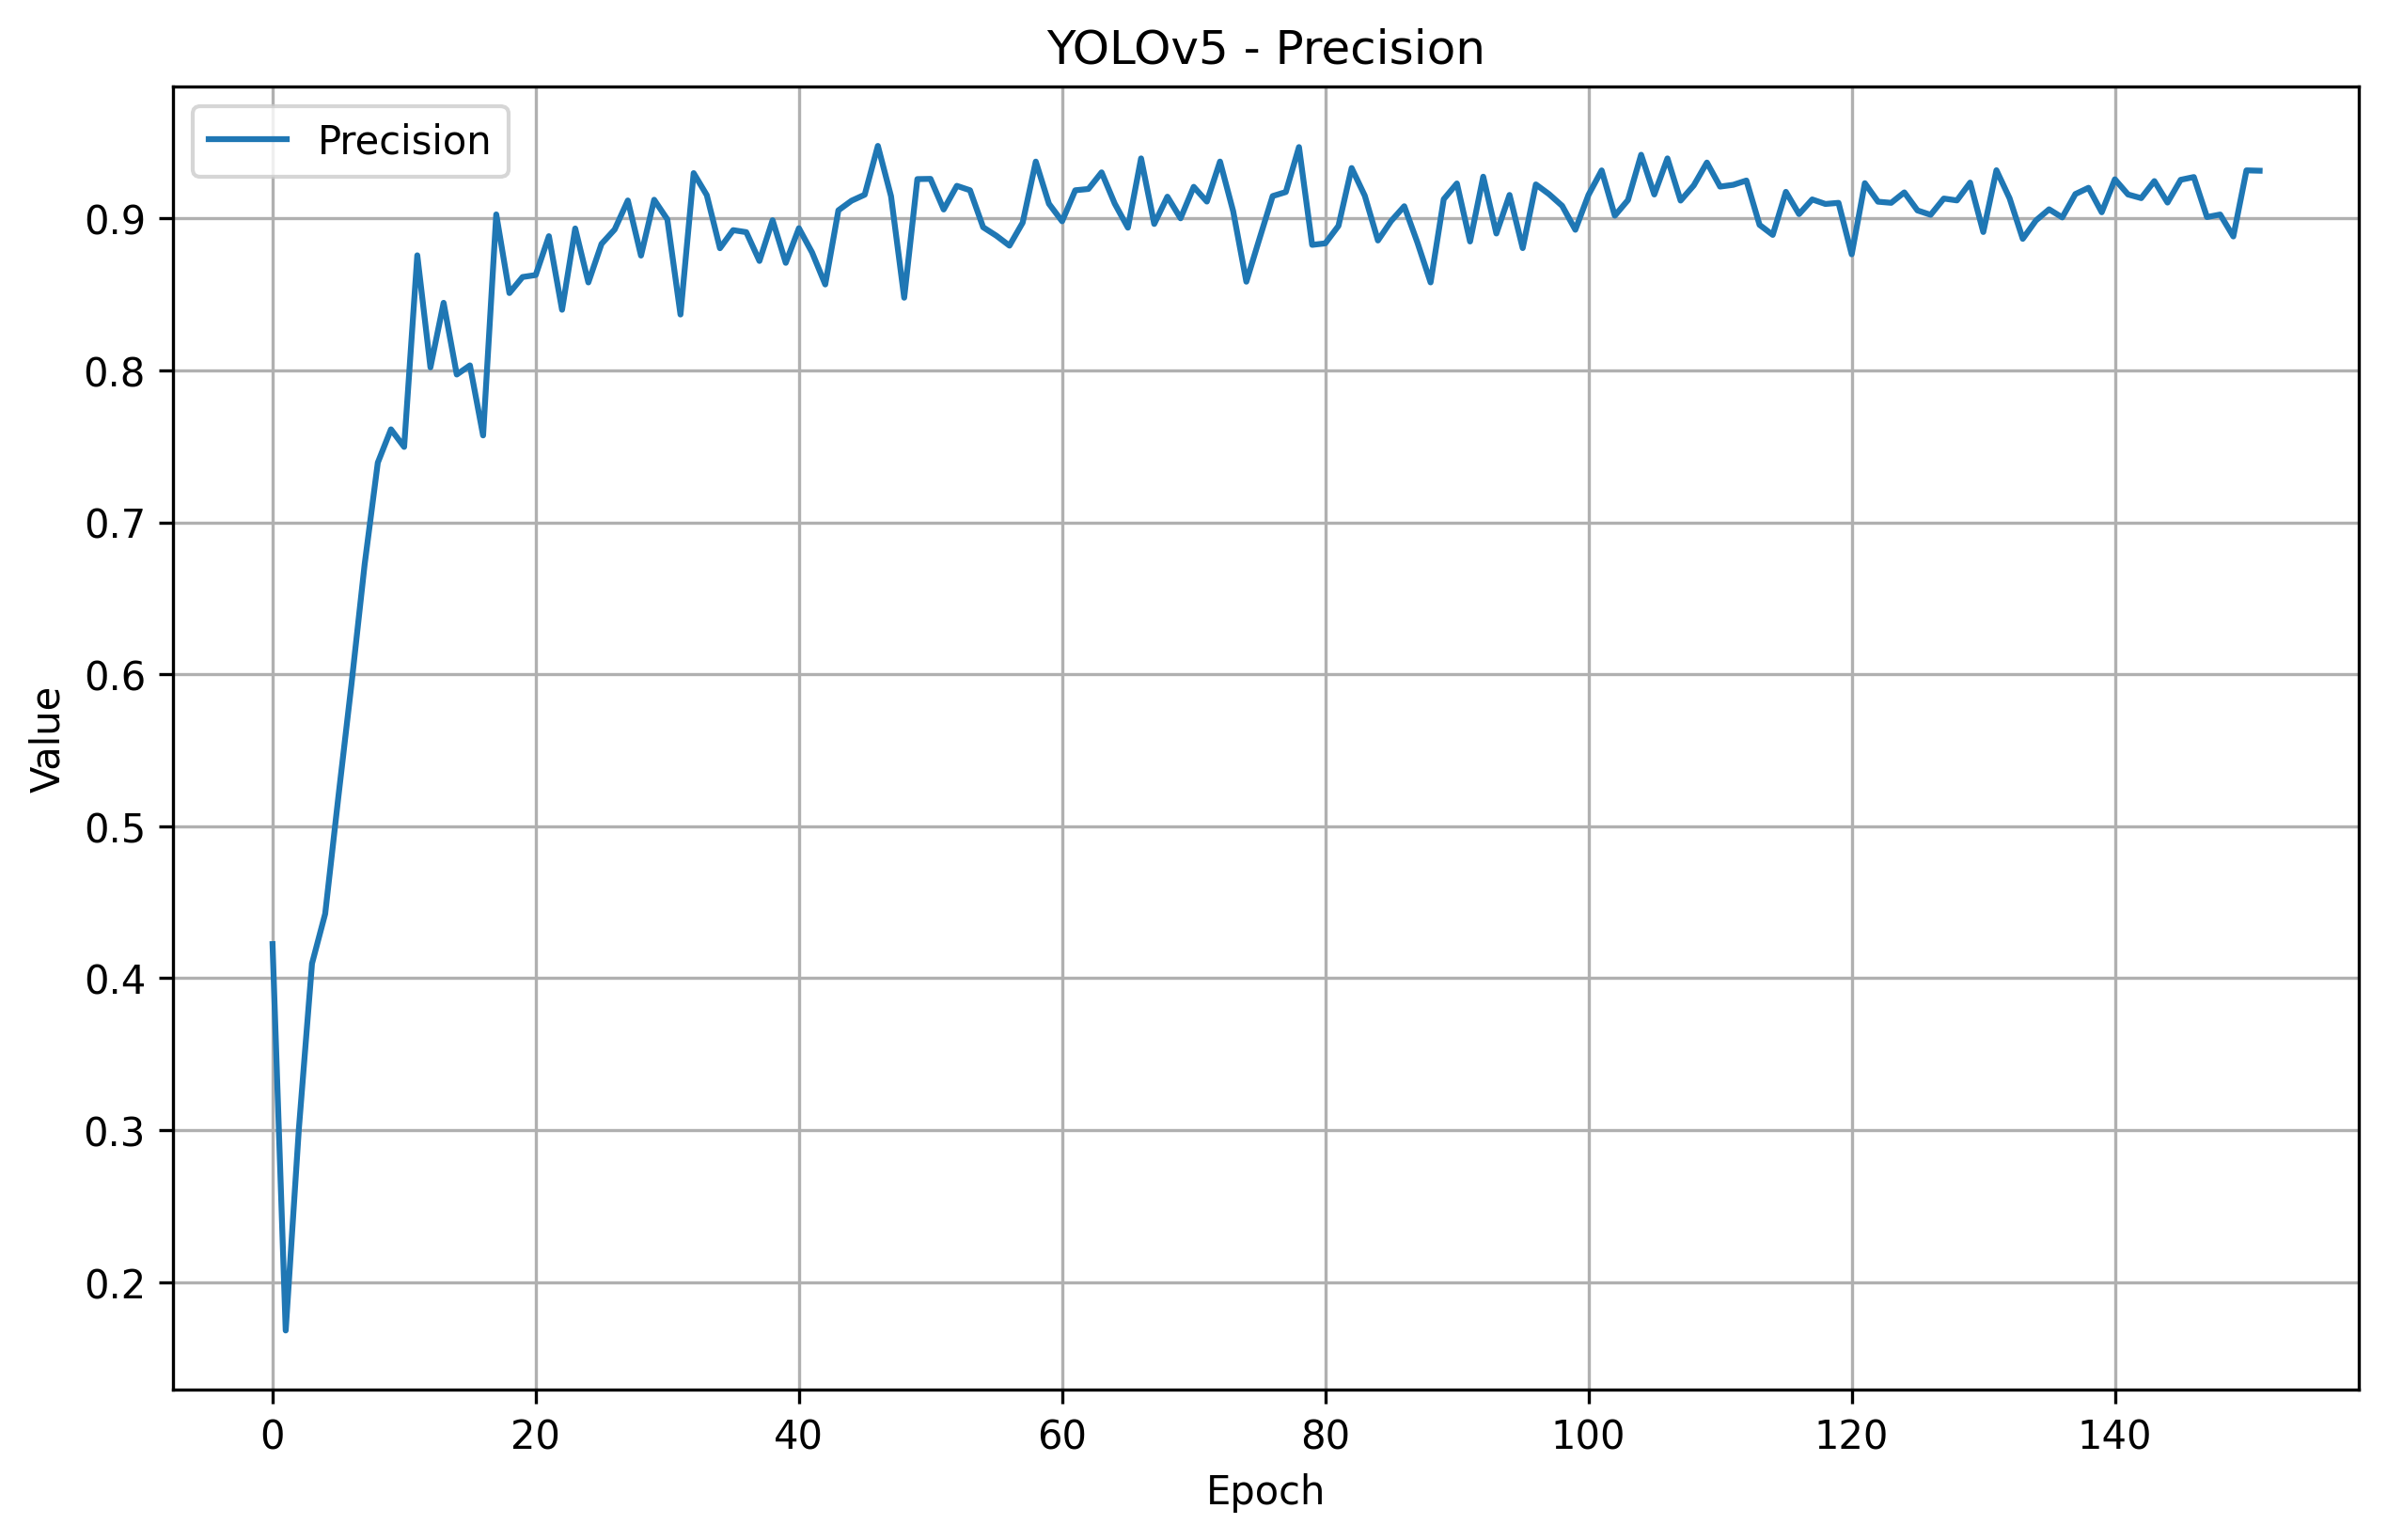
\includegraphics[width=\linewidth]{Precision.png}
    \caption{Box Loss}
  \end{subfigure}
  \begin{subfigure}[b]{0.495\textwidth}
    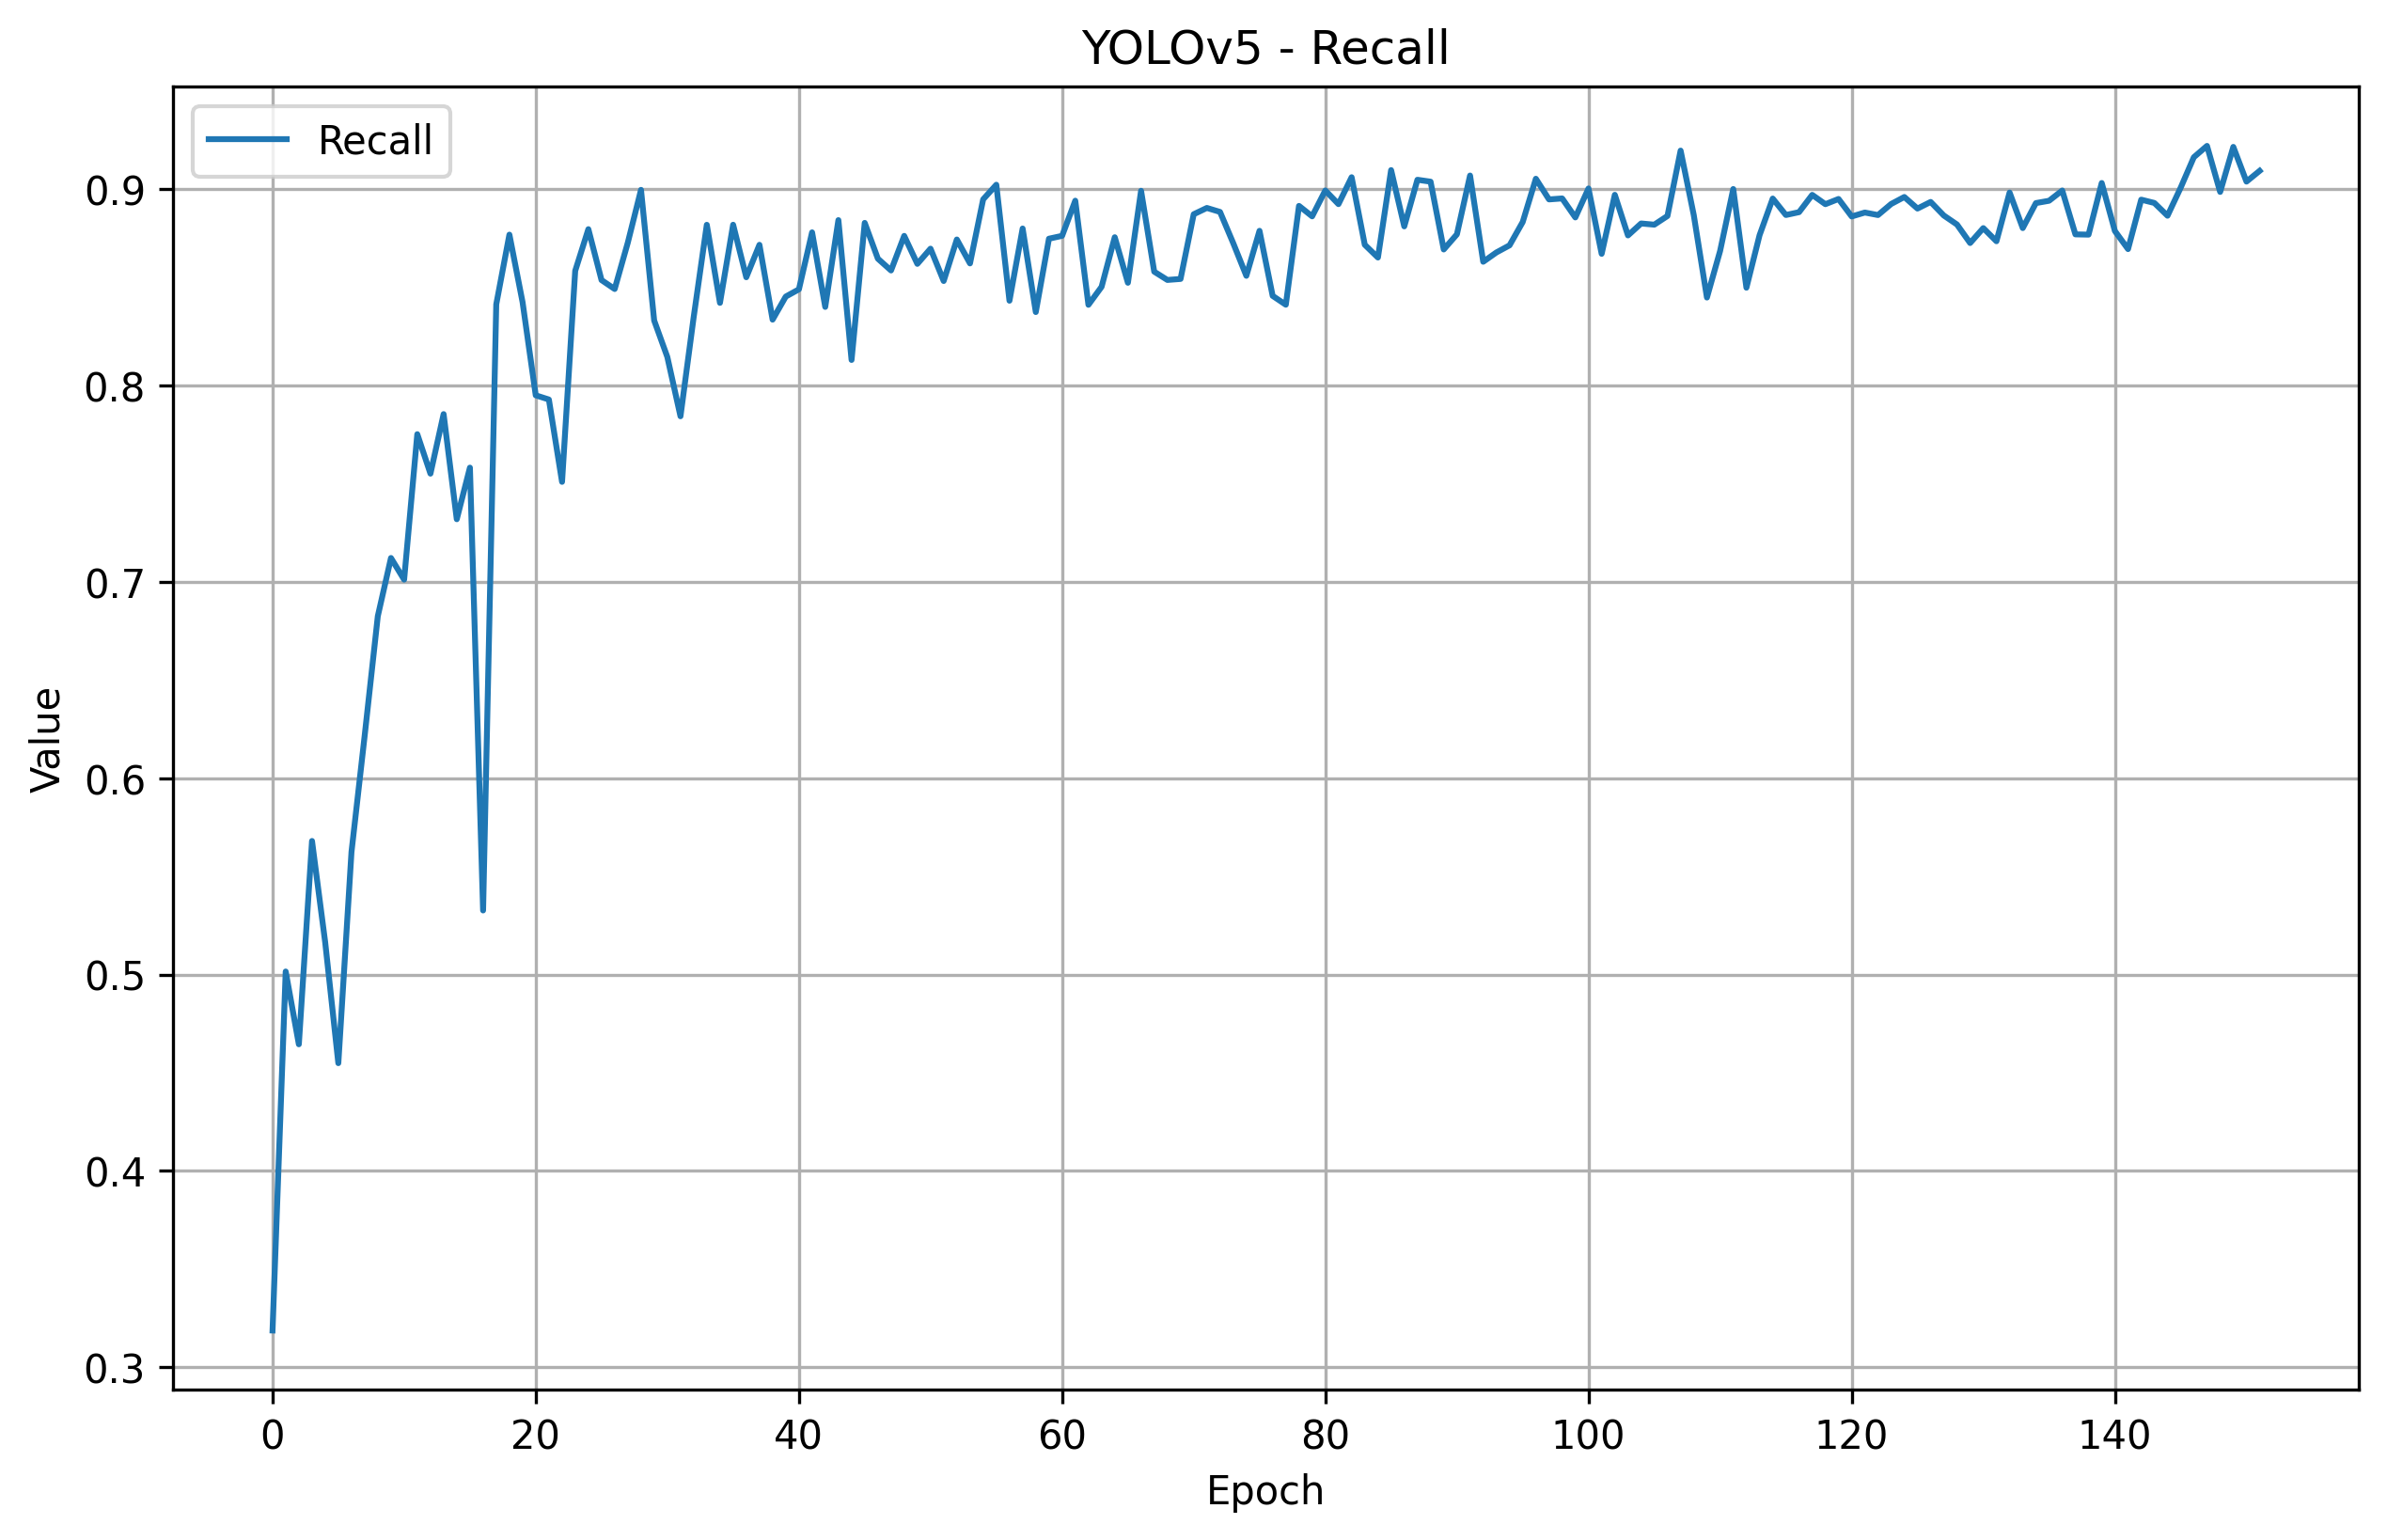
\includegraphics[width=\linewidth]{Recall.png}
    \caption{Class Loss}
  \end{subfigure}
\end{figure}
% # inserire immagini relative a addestramento precisione ecc

    \subsubsection{Object Detection}
    Come descritto precedentemente il modello si occupa di individuare un elemento stradale alla volta. In particolare per evitare confusioni con falsi positivi abbiamo deciso di salvare solo l'oggetto con maggiore confidenza. In futuro puntiamo a migliorare questo aspetto, in modo da poter salvare più oggetti contemporaneamente e prendere decisioni più complesse. Come ad esempio se il veicolo si trova davanti a un semaforo verde e un pedone, il veicolo dovrà fermarsi e dare la precedenza al pedone.
    Abbiamo utilizzato una formula chiamata \cite{distanza} Triangle Similarity per calcolare una stima della distanza tra il veicolo e l'oggetto individuato. Questa formula si basa sulla dimensione originale dell'oggetto in cm, la dimensione del bounding box in pixel e una distanza nota tra il veicolo e l'oggetto. In questo modo è possibile calcolare la distanza focale (La distanza tra il centro della lente (o l'obiettivo della fotocamera) e il punto focale, dove i raggi di luce paralleli convergono dopo essere passati attraverso la lente) e successivamente la distanza tra il veicolo e l'oggetto individuato.  
    \[
    \text{Distanza focale} = \frac{\text{Larghezza (px)} \times \text{Distanza nota (cm)}}{\text{Larghezza reale (cm)}}
    \]
    \[
    \text{Distanza (cm)} = \frac{\text{Larghezza reale (cm)} \times \text{Distanza focale}}{\text{Larghezza (px)}}
    \]

    Grazie a questo calcolo siamo in grado di stabilire una distanza ottimale per inviare il comando. La lente della PiCamera ha un FOV (Field of View) di 62.2 gradi, non è quindi in grado di individuare oggetti a distanze molto ravvicinate. Un cartello al lato della strada già a 10 cm di distanza non è più nell'inquadratura. Per questo motivo è stato necessario inviare il comando prima ed introdurre un delay in Arduino in modo da far fermare il veicolo (o cambiare la velocità) ad una distanza ottimale e realistica. 
    % inserire screenshot di segnale stop individuare e far vedere distanza calcolata devi anche verificare a che distanza non lo vede piu
    Infine abbiamo notato che essendo un modello molto piccolo YoloV5s non è estremamente preciso, abbiamo notato che molto spesso per pochi frame la classe scompare per poi essere di nuovo individuata. Per questo motivo abbiamo introdotto un timer di tolleranza. Ad esempio se per 30 frame consecutivi (circa 1 secondo) il modello non individua nulla o individua un'altra classe, non invierà alcun comando. Allo scadere del timer, verrà presa in considerazione ogni nuovo comando.
    

    
\subsection{Lane Detection}
Il controllo della direzione viene calcolato in contemporanea con l'object detection nel thread principale. Abbiamo convertito in scala di grigi il frame e tracciato una linea orizzontale. Questa riga parte dal centro e si estende a tutto il lato destro, per ogni pixel andiamo a rintracciare la striscia bianca in base all'intensità. Basandosi sulla posizione rilevata verrà stabilito se si dovrà effettuare la svolta o continuare dritto. Abbiamo impostato un range di pixel (rappresentato dalla linea bianca) che indica che il veicolo è posizionato correttamente e deve quindi procedere dritto. 
% Inserire screenshot destra sinistra e dritto

\textbf{Nota:} I comandi di direzione non sovrascrivono quelli dell'object detection. In questo modo una volta ferma allo stop l'analisi della corsia riprenderà solo se verrà dato il comando di ripartenza. 


\section{Sviluppi futuri del progetto}
\begin{enumerate}
\item Migliorare il comparto Hardware sostituendo il Pi Z2W con un Pi 4/5 in combinazione con una camera con FOV maggiore. In questo modo la macchina sarà del tutto autonoma poichè il modello girerà direttamente sul Raspberry.
\item Implementare una lane detection più complessa:
    \begin{itemize}
    \item Prenda in considerazione entrambe le strisce di corsia.
    \item Calcoli un valore di intesità di svolta.
    \end{itemize}
\item Ottimizzare l'alimentazione in un'unica soluzione.
\end{enumerate}

\newpage

\medskip


\printbibliography


\end{document}



